
% android_app.tex

\chapter{Android-App: ApoCo}

Dieses Kapitel besch\"aftigt sich mit der Android-Anwendung.
Hier werden im Folgenden Designentscheidungen in der Architektur, GUI und Implementierung beschrieben.
Au\ss{}erdem werden wichtige Hintergrundprozesse wie Bluetooth und die REST-Schnittstelle erl\"autert.\\




\section{Modellierung}

Die Software ist stark modularisiert und dom\"anenorientiert aufgebaut.
Wichtige Aspekte, die zu dieser Entscheidung gef\"uhrt haben, sind unter anderem,
dass die Software sp\"ater einfach und schnell erweitbar, \"anderbar und partiell wiederverwendbar sein soll.
Die Modularisierung erfolgt nach Funktionen und Teilaufgaben innerhalb einer Funktion.
ApoCo wird mittels verschiedener Architekturen realisiert.
Zun\"achst ist die grobe Struktur der Android-Anwendung als \emph{Model-View-Controller (MVC)} modelliert.
Die einzelnen Schichten Model, View und Controller der Android-Anwendung sind wie in der Abbildung 4.1 aufgeteilt.\\

\begin{figure}[h]
  \centering
  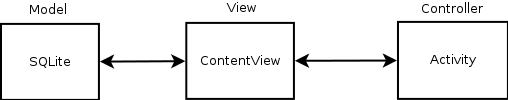
\includegraphics[scale=0.7]{diagramme/kapitel4/MVC.png}
  \caption{MVC-Architektur der ApoCo-Anwendung}
 
\end{figure}

\begin{itemize}
 \item Model: Die Model-Schicht ist die interne Datenbank der ApoCo-Anwendung.
 Als Datenbank nutzt Android SQLite.
 Dabei ist die Datenbank als eine Datei umgesetzt.
 Diese ist auf dem Dateisystem in Ordnern der ApoCo-Anwendung hinterlegt.
 Die Anfragen und Statements werden hier genauso verwendet wie das zum Beispiel der Fall bei MySQL oder Oracle Datenbanken ist.
 
 \item View: Die View-Schicht wird durch die \emph{Views} einer Android-Activity repr\"asentiert.
 Eine solche View wird in den meisten F\"allen in einer XML-Datei beschrieben.
 Diese Datei enth\"alt die Struktur einer View, welche dem Benutzer anschlie\ss{}end auf dem Bildschirm pr\"asentiert wird.
  
 \item Controller: Die Controller-Schicht wird durch die Anwendungslogik in den Activities umgesetzt.
 Hier wird die Interaktion des Patienten mit ApoCo abgefangen und die Ausgaben f\"ur den Bildschirm gesteuert.
\end{itemize}


Wird das gesamte Projekt betrachtet, handelt es sich dabei um eine Client-Server-Architektur.
In der Abbildung 4.2 wird die Aufteilung der einzelnen Software-Komponenten der Client-Server-Architektur dargestellt.\\

\begin{figure}[h]
  \centering
  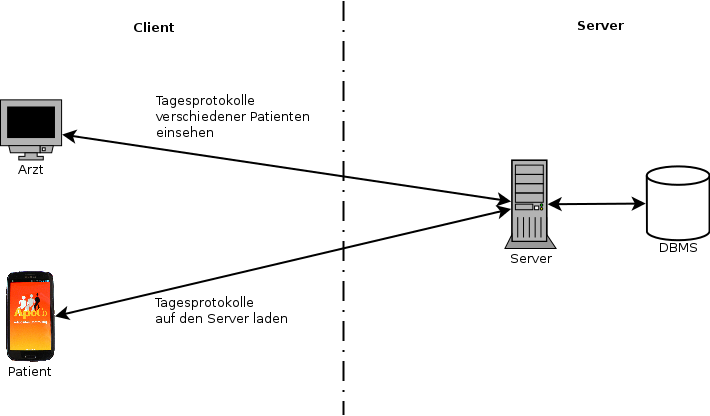
\includegraphics[scale=0.5]{diagramme/kapitel4/client_server.png}
  \caption{Client-Server-Architektur des gesamten Projekts}
  
\end{figure}

ApoCo ist der Teil der gesamten Software, welcher sich um das Aufzeichnen von Tagesprotokollen k\"ummert.
Um die Daten auswerten zu k\"onnen, benutzt der Arzt eine Webanwendung.
Dabei werden die Tagesprotokolle von der Datenbank geladen und im Webbrowser des Arztes angezeigt.\\
 



\section{Apoco Projektstruktur}

Die Abbildung 4.3 veranschaulicht die Paketstruktur der ApoCo-Anwendung.
Sie spiegelt die Modularisierung der ApoCo-Anwendung wieder.
Im Ordner \emph{src} befindet sich der gesamte Quellcode der Anwendung. 
Dieser liegt aufgeteilt in den jeweiligen Modul-Paketen im Hauptpaket der Anwendung \emph{com.janas.apoco}.\\

\subsection*{Paket activity}

Das Paket \emph{activity} beinhaltet alle f\"ur die ApoCo-Anwendung notwendigen Activities.
In diesem Paket befinden sich folgende Klassen:

\begin{itemize}
 \item ActivityBloodpressure:\\
 Hier steht die gesamte Anwendungslogik f\"ur das Protokollieren von Blutdruck.
 Die Activity veranschaulicht in einer scrollbaren Liste alle vorhandenen Messungen.
 Dar\"uber hinaus werden die Daten beim Verlassen der Activity \"uber das Internet mit einem Webserver synchronisiert. 
 
 \item ActivityBodyweight:\\
 Diese Activity behandelt das Protokollieren von K\"orpergewicht des Patienten und beinhaltet die daf\"ur notwendige Anwendungslogik.
 Auch hier werden in einer Listenansicht alle get\"atigten Messungen angezeigt.
 Beim Beenden der Activity werden die Protokolle mit einem Webserver synchronisiert.
 
 \item ActivityDeviceList:\\
 Diese Activity ist notwendig f\"ur das Koppeln \"uber Bluetooth von Sensoren mit dem Smartphone.
 Es ist eine von zwei M\"oglichkeiten des Koppelungsvorgangs in der ApoCo-Anwendung.
 Hier verh\"alt sich das Smartphone wie ein Client.
 Die Activity hat zwei Listen.
 In der einen Liste werden bereits bekannte Ger\"ate aufgelistet.
 Nach einem erfolgreichen Suchvorgang werden die gefundenen Ger\"ate in der zweiten Liste angezeigt.
 Man w\"ahlt aus einen der Listen das gew\"unschte Ger\"at zum Koppeln aus und sie verbinden sich untereinander.
 
 \item ActivityDevices:\\
 Diese Activity bietet die M\"oglichkeit den Koppelungsvorgang zu starten.
 Man w\"ahlt die Art des Messger\"ats aus, zum Beispiel K\"orperwaage, Blutdruckmesser oder Lebensmittelwaage.
 Anschlie\ss{}end w\"ahlt man die Koppelungsart aus.
 Zur Auswahl stehen die M\"oglichkeiten \emph{als Server} und \emph{als Client} zur Verf\"ugung.
 Die Methode \emph{pairing als Client} wird mittels der Klasse ActivityDeviceList ausgef\"uhrt.
 Die Methode \emph{pairing als Server} erledigt die ActivityDevices selbst.
 Daf\"ur startet sie einen Thread mit einem BluetoothServerSocket.
 Dieser h\"ort auf Anfragen von externen Ger\"aten zum Koppeln.

 \item ActivityFoodKcal:\\
 Hier wird der Benutzer drauf aufmerksam gemacht, wieviele Kilokalorien er am aktuellen Tag bereits zu sich genommen hat.
 Zus\"atzlich wird die erlaubte Restmenge berechnet und dem Benutzer angezeigt.
 Wird die erlaubte Tagesdosis \"uberschritten, erscheint eine Warnung auf dem Display.
 In einer Liste werden vorhergehende Mahlzeiten aufgelistet.
 Beim Klicken auf eine Mahlzeit wird die Activity \emph{ActivityMealenergyDetails} als \emph{Dialog} eingeblendet und listet die einzelnen
 Positionen der Mahlzeit mit Informationen \"uber Energie und Gewicht auf.
 Von hier aus gelangt der Benutzer weiter zur Protokollierung einer neuen Mahlzeit und zur Ger\"ate-Koppelung.
 
 \item ActivityMealenergy:\\
 Beim Start ist die Activity immer leer.
 Der Benutzer st\"o\ss{}t von hier aus den Protokollierungsvorgang an.
 \"Uber den Barcode-Button startet der Benutzer eine Activity f\"ur das Scannen von EAN-Codes.
 Anschlie\ss{}end wird eine interne und externe Datenbank nach der gescannten EAN-Nummer durchgesucht.
 Wird ein Eintrag gefunden, so wird der Benutzer zur Activity \emph{ActivityMealContent} weitergeleitet, sonst wird eine Fehlmeldung ausgegeben, dass das Lebensmittel
 nicht identifiziert werden konnte.

 \item ActivityMealenergyContent:\\
 In diese Activity gelangt man nur, wenn das Lebensmittel in der Datenbank identifiziert wurde. 
 Hier werden Detailinformationen \"uber das Lebensmittel angezeigt 
 und \"uber den Button \emph{Waage verbinden?} kann eine Verbindung zur Lebensmittelwaage ge\"offnet werden. 
 
 Nach erfolgreicher W\"agung errechnet die Activity die Energiemenge des gewogenen Lebensmittels, 
 die Gesamtenergie aller Mahlzeiten und
 die noch zur Verf\"ugung stehende Energiemenge f\"ur den aktuellen Tag.

 \item ActivityMealenergyDetails:\\
 Diese Activity erscheint lediglich im Stil eines \emph{Dialog}.
 Das bedeutet, dass die alte Activity im Hintergrund sichtbar bleibt  
 und der modale Dialog tritt wie ein Pop-up in den Vordergrund. 
 Sie besteht nur aus einer scrollbaren Liste und zeigt Details einer Mahlzeit auf.
%  \item ActivityFoodKcalNewEntry:\\

 \item ActivityLogin:\\
 Diese Activity dient dem Anmelden in der ApoCo-Anwendung.
 Alternativ kann ein neuer Benutzer zur Activity \emph{ActivityRegister} wechseln, um sich zu registrieren. 
 
 \item ActivityRegister:\\
 Die Activity tritt als modaler Dialog auf und dient der Erfassung eines neuen Benutzers.
 Hier tr\"agt der Benutzer seine Daten wie Vor- und Nachname, Email und Passwort ein.
 Die Activity f\"uhrt eine Plausibilit\"atskontrolle durch.
 Anschlie\ss{}end sendet sie die Daten an einen Webserver, welcher \"uberpr\"uft, 
 ob der Benutzername bereits vergeben ist. 
 Sollte der Name zur Verf\"ugung stehen, wird der Benutzer in die Datenbank aufgenommen, 
 andernfalls wird er abgelehnt. 
 Die Activity reagiert auf die Serverantwort und akzeptiert entsprechend die Benutzerdaten 
 oder fordert ihn erneut auf seine Eingabe zu \"uberarbeiten.
 
 \item ActivityServerOptions:\\
 Diese Activity erscheint als modaler Dialog und nimmt lediglich die Adresse und Port des Webservers entgegen.
 
 \item ActivitySplashscreen:\\
 Das Splashscreen wird beim Start von ApoCo f\"ur wenige Sekunden angezeigt.
 Diese Activity pr\"asentiert das Logo und den Schriftzug \emph{(Adipositas Controlling}.
 Die Activity beendet sich nach einem Timerablauf automatisch und startet die Start-Activity von ApoCo.

 \item ActivityStart:\\
 Das ist die Hauptactivity in der ApoCo-Anwendung.
 Hier w\"ahlt man die Art der Protokollierung aus.
 Das kann zum Beispiel eine K\"orpergewichtsmessung, Blutdruckmessung oder das Protokollieren der eigenen Nahrungsaufnahme sein.
 Dar\"uber hinaus hat der Benutzer von hier aus den Zugriff auf die Funktion zum Koppeln von Messsensoren.

 %  \item ActivitySummary:\\
\end{itemize}



\begin{figure}[h]
  \centering
  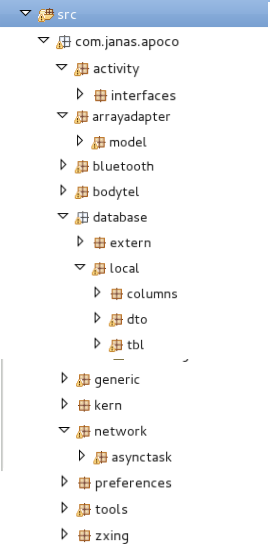
\includegraphics[scale=0.7]{screenshots/kapitel4/projekt_struktur/projekt_struktur_pakete.png}
  \caption{Projekt-Paketstruktur der ApoCo-Anwendung}
  
\end{figure}

\subsection*{Paket interfaces}

Das Paket \emph{activity} beinhaltet au\ss{}erdem das Unterpaket \emph{interfaces}.
Hier befinden sich Java-Schnittstellen, 
welche das Zusammenspiel zwischen Activities und Objekten f\"ur Anwendungslogik unterst\"utzen.
Diese Schnittstellen geben, au\ss{}er einigen Konstanten, auch Objektmethoden vor und werden f\"ur Polymorphie benutzt.
Folgende Interfaces liegen im Paket vor:

\begin{itemize}
 \item AccessableCreatorIF:\\
 Dieses Interface dient zum Erzeugen von unterschiedlichen Threads zur Kommunikation zwischen Software und externen Sensoren.
 F\"ur jeden Sensor steht ein angepasster Thread zur Kommunikation bereit.
 \"Uber dieses Interface wird immer das richtige Objekt durch die jeweilige Activity erzeugt und weitergereicht.

 \item ActivityExtrasCodesIF:\\
 In Android ist es m\"oglich Objekte oder einzelne Werte zwischen den Activities auszutauschen.
 Daf\"ur sind in diesem Interface Konstanten zum Zugriff auf die Daten bereitgestellt, 
 die \"uberall in der ApoCo-Anwendung zwischen den Activities ausgetauscht werden.
 
 \item ActivityRequestCodesIF:\\
 Soll aus einer Activity eine weitere gestartet werden und erwatet man von dieser ein Ergebnis, 
 so wird bei diesem Vorgang ein \emph{RequestCode} mitgegeben.
 Nach Ablauf einer Aufgabe kehrt eine Antwort zur urspr\"unglichen Activity mit dem Ergebnis und \emph{RequestCode} zur\"uck.
 Mit diesem RequestCode kann die Activity unterscheiden welche Antwort sie gerade bekommen hat.
 
 \item CloseableIF:\\
 Eine Activity, die dieses Interface implementiert, darf zum Beispiel von einem Thread oder \emph{Handler} geschlossen werden.
%  \item MessageDisplayableIF:\\
 \item WriteToPerformableIF:\\
 Dieses Interface muss von einer Activity implementiert werden, wenn sie eine Nachricht \"uber Bluetooth versenden muss.
 Die Nachricht wird an ein Thread \"ubergeben und dieser schreibt sie dann in den Streaminput eines \emph{BluetoothSocket}.
\end{itemize}

\subsection*{Paket arrayadapter}

Im Paket \emph{arrayadapter} befinden sich Implementierungen von performanten ArrayAdaptern.
Werden Daten in einer ListView dargestellt,
so kann man sie bequem aus einem Container, 
mittels einem ArrayAdapter in die ListView laden.
Die meisten Listen in ApoCo benutzen keine Standarddarstellung von Daten in einer ListView,
sondern eine individuell zugeschnittene Version.
F\"ur diesen Zweck ben\"otigt man einen zugeschnittenen ArrayAdapter, dessen Funktionalit\"at implementiert werden muss.
Die eigenen ArrayAdapter sind in der Lage Daten zwischenzuspeichern, wenn durch die ListView hin und her gescrollt wird.
Diese Daten m\"ussen nicht mehr nachgeladen werden und das sorgt f\"ur bessere Performance.\\
Im Paket \emph{arrayadapter} befindet sich ein Unterpaket.
Hier werden \emph{Model-Klassen} hinterlegt.
Das sind Daten-Container, welche Informationen f\"ur genau eine Messung speichern.
Zus\"atzlich bietet jedes Model eine statische Methode zum Konvertieren von Datenobjekten in Model-Objekte an. 
Dabei werden die Datenobjekte aus der Datenbank gelesen. 
Jede ListView findet hier einen eigenen ArrayAdapter und das dazugeh\"orige Model.\\

\subsection*{Paket bluetooth}

In diesem Paket befinden sich Klassen und Interfaces, die sich um die Kommunikation \"uber Bluetooth k\"ummern.
\begin{itemize}
 \item AcceptThread:\\
 Diese Klasse ist ein Thread, der einen BluetoothServerSocket startet und auf ankommende Anfragen zur Kommunikation wartet.
 Das ist der erste Schritt von Kommuikationsaufbau.
 
 \item AccessableIF:\\
 \"Uber dieses Interface kommunizieren Activities mit Threads, welche eine BluetoothSocket-Verbindung halten.
 
 \item BluetoothManager:\\
 Der BluetoothManager soll die gesamte Bluetooth-Funktionalit\"at in einer Klasse vereinigen.
 Mit dem BluetoothManager-Objekt wird die Kommunikation aufgebaut, kontrolliert und beendet.
 
 \item ConnectingThread:
 Dieser Thread ist der zweite Schritt zur Kommunikation \"uber Bluetooth.
 Er \"offnet einen Socket zur Gegenstelle und sendet Daten zwischen der Gegenstelle und der Activity.
 
 \item HandlerMessageIF:\\
 Dieses Interface beinhaltet alle Konstanten f\"ur einen Nachrichtenaustausch \"uber einen Handler.
 Die Konstanten erm\"oglichen der Activity zu erkennen, wie sie mit der Nachricht umgehen soll.
 
 \item PairingThread:\\
 Das ist ein Thread, der keine Kommunikation aufbaut.
 Er wird nur ganz kurz f\"ur das Koppeln von Smartphone und einem Sensor genutzt.

 \item StandardUUIDsIF:\\
 Dieses Interface ist vorgesehen, um bekannte standardisierte UUIDs als Konstante bereitzustellen.
 
 \item StartableCanceableIF:\\
 Dieses Interface schreibt einem Thread vor, dass er von Au\ss{}en gestartet und beendet werden kann.
\end{itemize}

\subsection*{Paket bodytel}

Dieses Paket beinhaltet alle Klassen und Interfaces, die notwendig sind, um eine Kommunikation mit Ger\"aten
der Firma Bodytel herzustellen.
Im Augenblick werden die Sensoren WeightTel und PressureTel unterst\"utzt.

\begin{itemize}
 \item BloodpressureResult:\\
 Nach einer Blutdruckmessung wird aus dieser Klasse ein Objekt erzeugt und mit den Messwerten initialisiert.
 Das Objekt wird anschlie\ss{}end in ein Model- und DTO-Objekt konvertiert.
 Das Model-Objekt wird zum Anzeigen in einer ListView genutzt und das DTO-Objekt zum Speichern der Messdaten in der Datenbank.
 
 \item BodyTelUUIDsIF:\\
 Dieses Interface stellt Konstanten bereit, welche von der Firma BodyTel als UUIDs f\"ur die Bluetoothverbindung genutzt werden.
 
 \item BodyweightResult:\\
 Ein Objekt dieser Klasse wird genauso verwendet wie bereits bei der Blutdruckmessung beschrieben wurde, 
 nur dass der Messwert mit der K\"orpergewichtsmessung initialisiert wird.
 
 \item PressureTelConnectedThread:\\
 Dieser Thread baut ein BluetoothSocket zwischen Smartphone und dem PressureTel-Blutdruckmesser auf.
 
 \item PressureTelCreator:\\
 Eine Activity nutzt diese Klasse, um dem BluetoothManager mitzuteilen,
 dass beim Bluetooth-Verbindungsaufbau ein Thread zur Kommunikation mit dem PressureTel gew\"unscht wird.
 
 \item PressureTelMeasurementDecoder:\\
 Diese Klasse dekodiert eine Nachricht von dem Blutdrucksensor.
 Daf\"ur wird die Nachricht in eiem \emph{PressureTelSMS}-Objekt verpackt und alle Messungen,
 die in der Nachricht enthalten sind, als separate \emph{BloodpressureResult}-Objekte
 in einer \emph{List<BloodpressureResult>} zur\"uckgegeben.
 
 \item PressureTelMessageProtocol:\\
 Ger\"ate der Firma BodyTel kommunizieren \"uber eine Art Konversationsprotokoll.
 Um die Messwerte auszulesen, muss dieses Protokoll erf\"ullt werden.
 In diesem Interface werden die notwendigen Konstanten f\"ur die Kommunikation mit dem Sensor \emph{PressureTel} bereitgestellt.
 
 \item PressureTelMessageReader:\\
 Diese Klasse reagiert nach dem Protokoll auf die Anfragen bei der Kommunikation mit dem PressureTel-Blutdrucksensor.
 Sie nutzt die anderen PressureTel-Klassen, um eine Nachricht zu analysieren, auf sie zu antworten, 
 Messwerte aus dieser zu dekodieren und sie in einer Liste an die Activity weiterzugeben. 
 
 \item PresurreTelSMS:\\
 Diese Klasse ist eine Wraper-Klasse f\"ur eine SMS-Nachricht des PressureTel-Sensors.
 Ein Objekt von dieser Klasse wird mit einer SMS initialisiert und konvertiert diese in ein Format,
 dass in ApoCo verwendet werden kann.
 
 \item WeightTelConnectedThread:\\
 Mit diesem Thread wird ein BluetoothSocket zwischen K\"orperwaage und Smartphone ge\"offnet.
 
 \item WeightTelCreator:\\
 Mit Hilfe dieser Klasse erzeugt der BluetoothManager einen Thread, 
 der an die Kommunikation mit der WeightTel-K\"orperwaage angepasst ist.
 
 \item WeightTelMeasurementDecoder:\\
 Diese Klasse wird genutzt, um eine Nachricht der K\"orperwaage zu dekodieren.
 Der Vorgang entspricht dem Dekodierungsvorgang des bereits beschriebenen Dekodierungsvorgangs beim PressureTel-Sensor.
 
 \item WeightTelMessageProtocol:\\
 F\"ur die Kommunikation mit dem WeightTel-Sensor stehen hier die notwendigen Konstanten bereit.
 
 \item WeightTelMessageReader:\\
 Wie beim PressureTel-Sensor, verwaltet diese Klasse den Dekodierungsvorgang einer Messung f\"ur den WeightTel-Sensor.
 
 \item WeightTelSMS:\\
 Diese Klasse ist das zentrale Koppelungselement zwischen einer SMS-Nachricht des WeightTel-Sensors und einer Datenstruktur, 
 die f\"ur ApoCo verwendbar ist.
 
\end{itemize}

\subsection*{Paket Database}

Die Klassen und Schnittstellen in diesem Paket erm\"oglichen einen Zugriff auf die interne und externe Datenbank.
Im Unterpaket \emph{extern} befinden sich zwei Interfaces.
Auf dem Webserver befindet sich in einem bestimmten Verzeichnis die REST-Schnittstelle zum Zugriff auf den MySQL-Datenserver.
Die Schnittstelle \emph{ExternServerDIR} hat eine Konstante, in der das Verzeichnis abgespeichert ist.
F\"ur jede Funktionalit\"at der REST-Schnittstelle gibt es eine entsprechende PHP-Datei.
Im Interface \emph{\texttt{PHP\_URL\_IF}} befinden sich Konstanten mit den Namen der PHP-Dateien.
Zum Beispiel entspricht die Konstante \emph{\texttt{REGISTER\_USER}} der URL \emph{\texttt{register\_user.php}}.
Ruft ApoCo diese URL mit den notwendigen Parametern auf, so ist es m\"oglich einen neuen User im System anzulegen.
Im Unterpaket \emph{local} sind Interfaces und Klasse f\"ur die interne Datenbank auf dem Smartphone.
Das Paket beinhaltet weitere Unterpakete: \emph{column}, \emph{dto} und \emph{tbl}.
Dies geh\"ort zu einem objektorientierten Konzept zum Zugriff auf die Datenbank, welches im Kapitel 4.3 erl\"autert wird.
Des Weiteren enth\"alt das Paket \emph{local} die Klasse DBManagerLocal und das Interface DBManagerPreferencesIF.
Der DBManagerLocal dient jeder Activity als Zugriffsmanager auf die interne Datenbank.
Das Interface DBManagerPreferencesIF dient zum Erstellen und der Konfiguration der Datenbank f\"ur die ApoCo-Anwendung.\\

\subsection*{Paket generic}

In diesem Paket befinden sich drei Klassen f\"ur die Durchf\"uhrung einer W\"agemessung mit der Lebensmittelwaage.
\begin{itemize}
 \item GenericCreator:\\
 Diese Klasse erzeugt einen Thread zur Kommunikation zwischen einer Activity und der KERN PCB-Laborwaage.
 \item KcalConnectedThread:\\
 Dieser Thread baut einen BluetoothSocket mit der Waage auf und kommuniziert mit ihr.
 \item KcalResult:\\
 Diese Klasse repr\"asentiert einen Messwert.
 Er setzt sich aus dem Gewicht und Eigenschaften des gewogenen Lebensmittels zusammen.
 
\end{itemize}

\subsection*{Paket kern}

In diesem Paket ist nur die Klasse \emph{\texttt{KERN\_PCB\_MessageBuilder}} enthalten.
Die Kern-Laborwaage sendet eine Messung als Datenbl\"ocke, die in kurzen Zeitabst\"anden nacheinander empfangen werden.
Diese Datenbl\"ocke werden in der Klasse gesammelt, analysiert und anschlie\ss{}end ein Messwert extrahiert.
Nachdem dieser Vorgang abgeschlossen ist, kann eine Activity \"uber die Methode \emph{readMessage()} den Messwert auslesen.\\

\subsection*{Paket network}

Hier befinden sich alle Klassen und Schnittstellen, die f\"ur eine Kommunikation \"uber WLAN oder das Mobile-Netz 
notwendig sind.
\begin{itemize}
 \item \texttt{JSON\_TAG\_IF}:\\
 Diese Schnittstelle stellt alle \emph{tag}-Namen zur Verf\"ugung, 
 die bei einem Datenaustausch mit dem Webserver im JSON-Format genutzt werden.
 
 \item NetworkHandler:\\
 Diese Klasse ist ein Handler, der in jeder Activity genutzt wird, welche mit dem Webserver kommunizieren muss.
 Vor einem Datenaustausch wird \"uberpr\"uft, ob eine WLAN- oder Mobile-Netz-Verbindung besteht und ob der Webserver antwortet.
 Je nach Ergebnis reagiert der Handler und benachrichtigt den Benutzer, wenn der Server nicht erreichbar ist.
 Eine Activity kann von diesem Handler geschlossen werden.
 Dazu muss sie die Schnittstelle \emph{CloseableIF} implementieren und mit einem Flag best\"atigen.
 Durch die Schnittstelle kann sie beendet werden, aber erst mit dem Flag wird dies auch abh\"angig von der Situation angefordert.
\end{itemize}

Im Unterpaket \emph{asynctask} befinden sich Klassen, welche von der Klasse AsyncTask<T,T,T> abgeleited werden.
Es handelt sich dabei um Threads, die einen Teil der Arbeit im UI-Thread durchf\"uhren und den Hauptteil als Nebenl\"aufigkeit.
Mit diesen Threads wird je eine bestimmte Netzwerkfunktionalit\"at der ApoCo-Anwendung erledigt.\\

\subsection*{Paket preferences}

Dieses Paket beinhaltet den \emph{PreferencesManager} und eine Schnittstelle \emph{\texttt{APOCO\_PREFERENCES}}.
Der \emph{PreferencesManager} behandelt ApoCo-spezifische Parameter.
Normalerweise k\"onnen Werte in einer Datei oder Datenbank persistent gespeichert werden.
Shared Preferences ist eine weitere M\"oglichkeit in Android, 
anwendungsbezogene Werte als eine Art Schl\"ussel-Wert-Paar zu speichern.
Die Schnittstelle \texttt{APOCO\_PREFERENCES} beinhaltet alle Schl\"ussel f\"ur den Zugriff auf die Shared Preferences.\\

\subsection*{Paket tools}

Das Paket \emph{tools} beinhaltet Werkzeuge, die projekt\"ubergreifend n\"utzlich sein k\"onnen.

\begin{itemize}
 \item BloodpressureDiagnose:\\
 Diese Klasse bietet Funktionen, die eine einfache Interpretation von Blutdruckwerten \"ubernehmen.
 Man \"ubergibt Blutdruckwerte an die Methode \emph{performDiagnose()} und bekommt eine Aussage \"uber die Messung.
  
 \item BodyweightDiagnose:\\
 Diese Klasse errechnet die Differenz zwischen Dem Zielk\"orpergewicht und dem aktuellen K\"orpergewicht.
 
 \item ConnectivityTest:\\
 Mit dieser Klasse ist es m\"oglich durch den Aufruf der Methode \emph{isAnyNetworkReachable()} festzustellen,
 ob das Smartphone \"uber WLAN oder Mobile-Netz mit dem Internet verbunden ist.
 
 \item DateTemplateIF:\\
 Diese Schnittstelle enth\"alt verschiedene Datumsmuster als Konstanten f\"ur eine Konvertierung eines Datums in ein 
 gew\"unschtes Format.
 \item FloatPrecision:\\
 Diese Klasse \"uberpr\"uft einen Flie\ss{}kommawert, ob er in der N\"ahe der Zahl 0 liegt. 
 F\"ur den Test ist ein Epsilon f\"ur die Pr\"azision notwendig.
 
 \item HexConverter:\\
 Diese Klasse bietet mehrere Methoden an, um hexadezimal codierte Bytearrays in lesbare Strings umzuwandeln und umgekehrt.
 
 \item JSONParser:\\
 Diese Klasse erleichtert das Senden und Empfangen von JSON-Strings zwischen einer Anwendung und einem Webserver.
 Dabei ist es m\"oglich die HTTP-Methoden POST und GET zu benutzen.
 Die Serverantwort wird als JSON-Objekt zur\"uckgegeben.
 
 \item PasswordCheck:\\
 Diese Klasse \"uberpr\"uft, ob ein Passwort der gew\"unschten Vorgabe entspricht.
 Es wird die Mindestl\"ange und die wiederholte Eingabe des Passwortes gepr\"uft.
 
 \item ResourcesTools:\\
 Diese Klasse ist ein Wraper, um aus Android-Ressourcen eine String-Ressource zu lesen.
 
 \item TimeTools:\\
 Diese Klasse konvertiert einen Timestamp vom Typ Long in einen String mit dem Format \emph{dd-MM-yyyy HH:mm} und umgekehrt.
 
 \item Toasting:\\
 Diese Klasse erleichtert Informationen \"uber einen Toast anzuzeigen.
 Der hier ausgegebene Toast entspricht nicht den Standardvorgaben, sondern ist individualisiert.
 
 \item URLBuilder:\\
 Diese Klasse bietet die Methode \emph{getURL()} an.
 Mit dieser Methode wird aus Parametern und einem formatierbaren String eine vollst\"andige URL-Adresse zusammengef\"ugt.
\end{itemize}

\subsection*{Paket zxing}

Dieses Paket enth\"alt zwei Klassen.
\emph{IntentIntegrator} und \emph{IntentResult}.
Diese zwei Klassen sind notwendig, um eine externe Barcodescanner-Anwendung zu nutzen.
Die Anwendung wird mit der Unterst\"utzung dieser Klassen in die eigene Anwendung integriert 
und man erh\"alt Zugriff auf den Barcode als String. \\




\section{Architektur der ApoCo-Datenbank(SQLite)}

Im Buch von Arno Becker und Marcus Pant\cite[S.244]{Android:02}, wird ein Architekturvorschlag f\"ur eine
Datenbankzugriffsschicht f\"ur Android-Anwendungen gemacht.
ApoCo folgt diesem Vorschlag, der hier erl\"autert wird.

\subsection{Motivation}

Beim Umgang mit einer Datenbank ist es oft erw\"unscht eine von der Anwendungsschicht getrennte Zugriffsschicht auf die Datenbank zu haben.
Daf\"ur kann man sich an dem Konzept der Programmierung mit Java-EE orientieren.
Android ist f\"ur ein solches Konzept nicht ausgelegt und so ergeben sich folgende Nachteile:

\begin{itemize}
 
\item Die Anwendung wird ungewollt gro\ss{} und die Performance sinkt.
\item Da keine Frameworks, wie zum Beispiel Spring oder Hibernate existieren, sind \"Anderungen an der Datenbank sehr aufwendig.
\item Es gibt keine M\"oglichkeit die Datenbankschicht von der Pr\"asentationsschicht ohne sp\"urbaren Leistungsabfall zur Laufzeit zu trennen
\cite[S.244]{Android:02}.

\end{itemize}

Au\ss{}erdem wurde festgestellt, dass eine reine Schichtentrennung unm\"oglich ist, 
wenn man mit einem Cursor-Objekt arbeiten m\"ochte.
Der Cursor ist wie ein Zeiger und ist darauf ausgelegt mit gro\ss{}en Datenmengen in einer Datenbank umgehen zu k\"onnen.\\

\subsection{Architekturumsetzung}

Die Zugriffsschicht auf die Android-Datenbank besteht aus den folgenden Klassen:

\begin{itemize}
 \item DBManagerLocal
 \item TabellennameColumns
 \item TabellennameDTO
 \item TabellennameTbl
\end{itemize}

Dabei ist zu beachten, dass f\"ur jede Tabelle eine \emph{Columns, DTO} und \emph{Tbl}-Klasse existiert. 
Die Bezeichnung dieser Klassen setzt sich aus dem Tabellennamen als Pr\"afix und den so eben genannten Klassenendungen zusammen.\\

Die Klasse \emph{DBManagerLocal} ist eine Verwaltungsklasse, um die Datenbank in der Activity greifbar zu machen.
Diese Verwaltungsklasse erweitert die Klasse SQLiteOpenHelper aus dem Android-SDK.
Der SQLiteOpenHelper wei\ss{} wie eine Datenbank erzeugt und ge\"andert wird.
Daf\"ur sind zwei Methoden vorgegeben: \emph{onCreate()} und \emph{onUpgrade()}.
Mit diesen zwei Methoden wird das Datenbankschema aufgebaut und bei \"Anderungen gel\"oscht und neu aufgebaut.
Um einen Backup-Mechanismus muss man sich selbst k\"mmern.
Des Weiteren sind im \emph{DBManagerLocal} Methoden implementiert, um mit der Datenbank Daten auszutauschen.
Im Listing 4.1 wird eine reduzierte Version des \emph{DBManagerLocal} implementiert und es wird eine Tabelle \emph{user} angelegt.
Die Klasse \emph{DBManagerLocal} implementiert die Schnittstelle \emph{DBManagerPreferencesIF}.
In dieser Schnittstelle wird der Name der Datei f\"ur die Datenbank und die Versionsnummer hinterlegt.
Die Versionsnummer ist hier sehr wichtig.
Wird das Datenbankschema ge\"andert, so muss die Versionsnummer inkrementiert werden.
Nur so erkennt die Klasse SQLiteOpenHelper, dass die Datenbank neu aufgebaut werden muss.\\

\begin{lstlisting}[caption={Beispiel f\"ur reduzierte Implementierung der \emph{DBManagerLocal} Klasse}]
 public class DBManagerLocal extends SQLiteOpenHelper implements DBManagerPreferencesIF{ 
 
    public DBManagerLocal(Context context) {
       super(context, DATENBANK_NAME, null, DATENBANK_VERSION);
    } 
    public void onCreate(SQLiteDatabase db) { 
    }    
    public void onUpgrade(SQLiteDatabase db, int oldVersion, int newVersion) {
    }
 }
\end{lstlisting}

Die \emph{TabellennameColumns}-Klassen sind als Schnittstellen und werden pro Tabelle angelegt.
Sie besitzen Konstanten f\"ur jede Spaltenbezeichnung der jeweiligen Tabelle.
Im Listing 4.2 wird ein Beispiel \emph{Columns-Klasse} f\"ur die Tabelle \emph{user} veranschaulicht.\\

\begin{lstlisting}[caption={Die Schnittstelle \emph{UserColumns}}]
 public interface UserColumns {
     static final String _ID      = "_id";
     static final String VORNAME  = "vorname";
     static final String NACHNAME = "nachname";
     static final String EMAIL    = "email";
     static final String PASSWORD = "password";
 }
\end{lstlisting}

Beim Zugriff auf die Tabelle \emph{user} wird im SQL-Statement \"uber die Konstanten der \emph{Columns-Klasse} auf die 
einzelnen Tabellenspalten zugegriffen.
In der Klasse \emph{TabellennameTbl} werden Schemainformationen und SQL-Statements als Konstanten vom Typ String bereitgestellt.
Die Klasse \emph{DBManagerLocal} nutzt die Schemainformationen, um eine Tabelle zu erzeugen.
Die SQL-Statements sind als Prepared Statements zu verstehen.
Das bedeutet, dass sie nur ein SQL-Statement-Muster ohne Parameter repr\"asentieren.
F\"ur Parameter wird das Fragezeichen (\emph{?}) als Platzhalter verwendet, 
das vor dem Zugriff auf die Datenbank durch einen echten Parameter ersetzt wird.
Das Listing 4.3 veranschaulicht mit der \emph{UserTbl} eine Tabellenschema-Klasse.\\

\begin{lstlisting}[caption={Die Klasse \emph{UserTbl}}]
 public final class UserTbl implements UserColumns {
 
    //Tabellenname
    public static final String TABLE_NAME = "user";
    
    //Create-Statement zum Anlegen der Tabelle
    public static final String SQL_CREATE = 
       "CREATE TABLE " + TABLE_NAME + "(" + 
      _ID + " INTEGER PRIMARY KEY AUTOINCREMENT," + 
      VORNAME + " TEXT NOT NULL," + 
      NACHNAME + " TEXT NOT NULL," + 
      EMAIL + " TEXT NOT NULL," + 
      PASSWORD + " TEXT NOT NULL" + ");";
      
   //Drop-Statement zum L\"oschen der Tabelle
   public static final String SQL_DROP = 
      "DROP TABLE IF EXISTS " + TABLE_NAME;
      
   //Beispiel-Statement, welches alle Benutzer mit dem gleichen Nachnamen zurueckgibt.
   //Der Nachname wird als Parameter uebergeben.
   public static final String STMT_GET_USER = 
      "SELECT * FROM " + TABLE_NAME + 
      "WHERE " + NACHNAME + "=?";
}
\end{lstlisting}

Listing 4.4 zeigt ein Beispiel, um die Tabelle \emph{user} zu erzeugen oder sie bei \"Anderungen des Datenbankschemas neu zu erzeugen.
Daf\"ur ruft die \emph{DBManagerLocal}-Klasse die Methode \emph{onCreate()} bzw. \emph{onUpgrade()} automatisch auf.\\

\begin{lstlisting}[caption={\emph{DBManagerLocal} erzeugt die Tabelle \emph{user}}]
 public void onCreate(SQLiteDatabase db) {  
    //erzeuge user-Tabelle
    db.execSQL(UserTbl.SQL_CREATE);
 }
    
 public void onUpgrade(SQLiteDatabase db, int oldVersion, int newVersion) {
    //loesche und erzeuge die user-Tabelle
    db.execSQL(UserTbl.SQL_DROP);
    onCreate(db);
 }
\end{lstlisting}

Beim Aufrufen des DROP- und CREATE-Statements muss wegen der Tabellenabh\"angigkeiten auf die richtige Reihenfolge geachtet werden.
Erstellt werden immer zuerst Tabellen ohne Fremdschl\"ussel und dann der Rest.
Die Tabellen werden in genau umgekehrter Reihenfolge wieder gel\"oscht.
Die \emph{TabellennameDTO}-Klassen sind einfache Container-Klassen und erm\"oglichen einen objektorientierten Umgang mit den Ergebnissen aus Datenbankanfragen oder 
das \"Ubergeben eines \emph{DTO}-Objekts an die Datenbank zum Speichern.
Im Listing 4.5 wird eine stark reduzierte \emph{DTO}-Klasse f\"ur die Tabelle \emph{user} veranschaulicht.
Die \emph{DTO}-Klassen haben Felder, die den Spalten der Tabelle entsprechen, welcher sie angeh\"oren.
Ein \emph{DTO}-Objekt kann auf verschiedene Arten entstehen.
Aus Parametern, die sich aus Messungen und Benutzereingaben ergeben, 
aus einer Datenbankanfrage, die einen Cursor liefert oder einem JSON-Objekt aus einer Anfrage an den Webserver.
Es kann auch notwendig sein ein Objekt mit einem Standardkonstruktor zu erzeugen und die Felder sp\"ater zu initialisieren.
F\"ur diese F\"alle werden vier Konstruktoren ben\"otigt.
Nicht jede \emph{DTO}-Klasse ben\"otigt immer alle vier Konstruktoren.\\

\begin{lstlisting}[caption={\emph{UserDTO}-Klasse in leicht reduzierter Form}]
public class UserDTO {

   public long _id;
   public String vorname;
   public String nachname;
   public String email;
   public String password;
   
   
   public UserDTO(){};
   public UserDTO(long, String, String, Sting, String){...}
   public UserDTO(Cursor){...}
   public UserDTO(JSONObject){...}
   //getter & setter
   
   public JSONObject toJSONObject() {... return jsonObj;}
}
\end{lstlisting}

Eine wichtige Methode jeder \emph{DTO}-Klasse ist die \emph{toJSONObject()}-Methode.
F\"ur den Fall, dass Messungen oder Benutzereingaben an den Webserver geschickt werden m\"ussen,
geschieht dies \"uber eine REST-Schnittstelle mit einem JSON-String.
Um es so einfach wie m\"oglich zu halten die Objekte als Parameter an die REST-Schnittstelle zu senden,
hat jedes Objekt die F\"ahigkeit seine gespeicherten Eigenschaften als ein JSON-Objekt zur\"uckzugeben.
Die Implementierung dieser Methode veranschaulicht das Listing 4.6.\\

\begin{lstlisting}[caption={\emph{UserDTO}-Klasse in leicht reduzierter Form}]
public class UserDTO {
   public JSONObject toJSONObject() {
      JSONObject obj = new JSONObject();
      try {
         obj.put(UserTbl._ID, this._id);
         obj.put(UserTbl.VORNAME, this.vorname);
         obj.put(UserTbl.NACHNAME, this.nachname);
         obj.put(UserTbl.EMAIL, this.email);
         obj.put(UserTbl.PASSWORD, this.password);
      } catch (JSONException e) {
         Log.d(CLAZZ_NAME, "toJSONObject failed: " + e.getMessage());
      }
      return obj;
   }
}
\end{lstlisting}
Das Listing 4.6 demonstriert auch gleichzeitig wie die \emph{Tbl}-, \emph{Columns}- und \emph{DTO}-Klassen zusammenarbeiten.
Um die richtige Spaltenbezeichnung zu nutzen, greift die \emph{DTO}-Klasse \"uber die \emph{Tbl}-Klasse auf die \emph{Columns}-Schnittstelle 
und dort auf die Konstanten der Spaltennamen zu.
Damit eine Activity mit dem \emph{DBManagerLocal} auf die Datenbank Zugriff bekommt, 
m\"ussen Methoden f\"ur den Zugriff in der Klasse \emph{DBManagerLocal} implementiert werden.
Im Listing 4.3 wird bereits das SQL-Statement \emph{\texttt{STMT\_GET\_USER}} in der \emph{UserTbl}-Klasse gezeigt.
Dieses Statement nutzt der \emph{DBManagerLocal} in einer eigenen Methode, um eine Anfrage daraus zu bauen.
Eine Beispielanfrage wird mit dem Listing 4.7 demonstriert.\\

\begin{lstlisting}[caption={Methode \emph{getUserByNachname()} der \emph{DBManagerLocal}-Klasse}]
public class DBManagerLocal ... {
   ...
   //Methode fuer eine Datenbankanfrage
   public Cursor getUserByNachname(UserDTO user) throws SQLException{
      //Hier wird der Nachname aus dem DTO-Objekt als Parameter in einem String-Array gespeichert.
      String[] param = {user.nachname};
      //getReadableDatabase liefert eine Referenz auf ein Objekt, welches die Datenbankverbindung zum Lesen oeffnet.
      //das Statement aus der Klasse UserTbl und die Parameter werden an die Methode rawQuery uebergeben.
      //rawQuery liefert einen Cursor auf die Antwort aus der Datenbank.
      Cursor cursor = getReadableDatabase().rawQuery(UserTbl.STMT_GET_USER, param);
      return cursor;
   }   
}
\end{lstlisting}

Das Ergebnis der Anfrage kann in einer Activity anschlie\ss{}end ausgewertet werden.
Eine Demonstration liefert das Listing 4.8.
Hier wird zuerst mit dem if-Statement gepr\"uft, ob ein Ergebnis in der Datenbank gefunden wurde.
Die while-Schleife bewegt beim ersten Durchlauf den Cursor auf die erste Zeile der Antwort.
Im Rumpf der while-Schleife werden die Ergebnisse bearbeitet, und das so lange bis die Methode moveToNext() ein false liefert.\\

\begin{lstlisting}[caption={Methode \emph{getUserByNachname()} der \emph{DBManagerLocal}-Klasse}]
public class MyActivity... {
   ...    
   DBManagerLocal dbManager = new DBManagerLocal(MyActivity.this);      
   
   public void todo() {         
      Cursor result = dbManager.getUserByNachname(user);      
      if (result.getCount() > 1) {      
         while(result.moveToNext()) {         
            UserDTO user = new UserDTI(result); ...
         }
      }
   }
}
\end{lstlisting}

\subsection{ApoCo Datenbankdiagramm}

In der Abbildung 4.4 wird das ApoCo Datenbankschema als Klassendiagramm dargestellt.
Die Abk\"urzungen \emph{FK1, FK2} stehen dabei f\"ur Fremdschl\"ussel. Die Prim\"arschl\"ussel werden als Schl\"usselsymbol dargestellt.
Folgende Tabellen sind im Diagramm zu sehen:

\begin{itemize}
 \item user:\\
 Diese Tabelle enth\"alt Daten der Patienten.
 Die ApoCo-Anwendung ist so konzipiert, dass sie mehrere Patienten auf einem Smartphone verwalten kann.
 Jeder Patient hat seine eigenen Anmeldedaten und kann die Daten der anderen Patienten nicht einsehen.
 
 \item bloodpressure:\\
 In dieser Tabelle werden Messprotokolle f\"ur den Blutdruck persistent gespeichert.
 Neben dem Datum und den Spalten f\"ur die Messwerte ist hier noch eine weitere Spalte mit der Bezeichnung \emph{sync} zu sehen.
 Diese Spalte ist f\"ur die Synchronisation der Daten mit dem Webserver norwendig.
 Es handelt sich dabei um einen Flag der von 0 auf 1 gesetzt wird, wenn die Messwerte an den Webserver \"ubertragen wurden.
 
 \item bodyweight:\\
 Die Tabelle \emph{bodyweight} speichert Messdaten zum K\"orpergewicht.
 Auch hier ist ebenfalls eine Flag-Spalte f\"ur den Synchronisationsvorgang.
 
 \item mealenergy:\\
 Die Tabelle \emph{mealenergy} repr\"asentiert pro Eintrag eine ganze Mahlzeit.
 Hier wird nur festgehalten wann die Mahlzeit eingenommen wurde und ob die Mahlzeit mit dem Webserver synchronisiert ist.
 
 \item \texttt{mealenergy\_content}:\\
 Diese Tabelle enth\"alt einzelne Positionen einer Mahlzeit.
 Sie speichert aber nur das Gewicht und die Energiemenge der jeweiligen Position, wie auch die dazugeh\"orige EAN-Nummer.
 Die Tabellen \emph{mealenery} und \emph{\texttt{mealenergy\_content}} bilden somit eine Einheit bei der Berechnung von Energieaufnahme 
 durch die Nahrung.
 
 \item food:\\
 Die Tabelle \emph{food} dient als Erg\"anzung der Positionen einer Mahlzeit.
 Jedes Lebensmittel, das zum ersten Mal mit Hilfe des Barcodescanners erkannt wurde, wird hier f\"ur schnellen Zugriff gespeichert.
 
 \item tageseinheiten:\\
 Der Arzt gibt seinen Patienten vor, wieviel Kilokalorien sie am Tag zu sich nehmen d\"urfen.
 Die aktuellen Werte werden vom Webserver geladen und in dieser Tabelle abgelegt.
\end{itemize}

\begin{figure}[h]
  \centering
  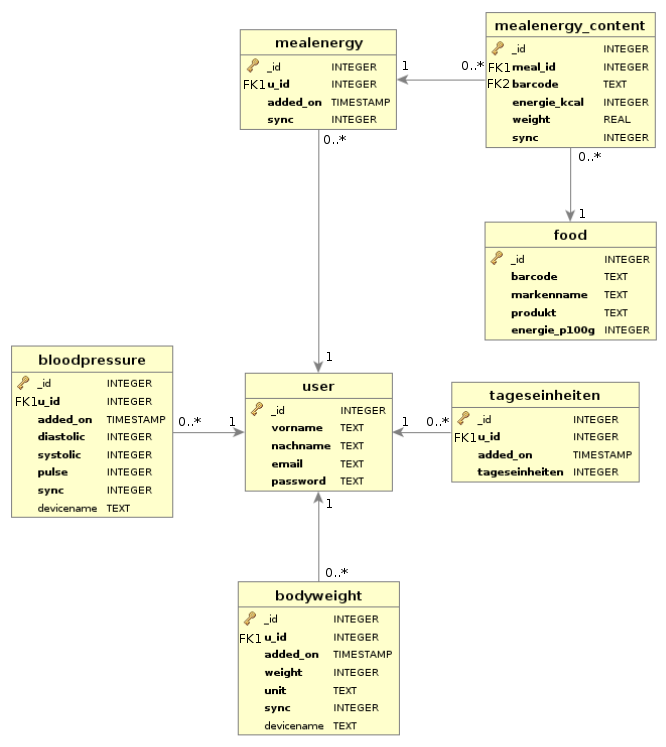
\includegraphics[scale=0.53]{diagramme/kapitel4/apoco_datenbank_schema.png}
  \caption{ApoCo Datenbankdiagramm}
  
\end{figure}




\section{Bluetoothkommunikation, Messung und Persistierung} 

Um Messdaten zu erhalten, kommuniziert ApoCo mit den Messsensoren \"uber Bluetooth.
Die eingesetzten Sensoren der Firma BodyTel verwenden f\"ur die \"Ubermittlung der Messdaten 
ein Protokoll, das dem \emph{PDU-Modus} einer SMS entspricht.
PDU steht f\"ur \emph{Protocol Data Unit} und ist eine von drei Spezifikationen, 
welche vom \emph{Europ\"aischen Institut f\"ur Telekommunikationsnormen} (ETSI)\cite{ETSI:01}
zum Standard f\"ur SMS-Nachrichten erkl\"art wurde.
In diesem Protokoll werden AT-Kommandos f\"ur den Verbindungsaufbau eingesetzt 
und anschlie\ss{}end die Messwerte im PDU-Modus \"ubermittelt. 
AT-Kommandos sind ein Befehlssatz, der zum Parametrieren und Konfigurieren von Modems genutzt wird\cite{AT-command:01}.
Mit einem AT-Kommando teilt der Messsensor der Software mit, wenn er im n\"achsten Schritt eine Nachricht \"ubermitteln m\"ochte.
Da jeder Messsensor nur f\"ur eine bestimmte Art von Messung geeignet ist, underscheiden sich die PDUs der einzelnen Ger\"ate.
Nach dem ein Sensor \"uber Bluetooth mit dem Smartphone gekoppelt ist und verwendet werden soll, muss ApoCo 
als Bluetooth-Server auf ankommende Nachrichten h\"oren.\\
Im Gegensatz zu der Bluetoothkommunikation der BodyTel-Ger\"ate wird bei der Verbindung mit der Laborwaage f\"ur das Abwiegen
von Lebensmitteln kein Kommunikationsprotokoll verwendet.
Die Waage kommuniziert \"uber eine RS-232-Schnittstelle direkt ohne die Nachricht zu kodieren.
An dieser Schnittstelle sitzt ein Bluetooth-Dongle und ersetzt ein serielles Kabel.
ApoCo baut eine BluetoothSocket-Verbindung zu der Bluetooth-Dongle Adresse auf.
Die Waage sendet die Messwerte im 8-Bit ASCII-Code. 
Was beim Wiegen an Daten gesendet wird, kann an der Waage parametriert werden.
F\"ur die Kommunikation mit ApoCo wird das gemessene Nettogewicht \"ubertragen.
Direkt nachdem eine Socketverbindung zwischen ApoCo und der Waage aufgebaut ist, 
k\"onnen Daten von der Waage im ASCII-Code empfangen werden.\\


\subsection{Bluetoothkommunikation BodyTel}

In der Abbildung 4.5 wird am Beispiel der K\"orpergewichtsmessung demonstriert,
wie ein Verbindungsaufbau und Datenaustausch zwischen ApoCo und der K\"orperwaage zustande kommt.
Nach dem Start initialisiert die Activity \emph{ActivityBodyweight} den \emph{BluetoothManager} 
und erzeugt ein Objekt vom Typ \emph{WeightTelCreator}.
Anschlie\ss{}end wird die Methode \emph{listenForInquiryConnections()} des \emph{BluetoothManager} gerufen.
Dabei \"ubergibt die Activity der Methode ein Objekt vom Typ Handler und \emph{WeightTelCreator}.
Der Handler ist zust\"andig f\"ur Intraprozesskommunikation zwischen der Activity und einem Thread.
Kommt eine Nachricht \"uber den BluetoothSocket rein, so kann diese nicht direkt an die Activity gegeben werden.
Das kann der Thread nur \"uber den Handler tun.
Der \emph{WeightTelCreator} erzeugt den Thread und gibt eine Referenz auf ihn zur\"uck.
Die Referenz ist eine Schnittstelle vom Typ \emph{AccessableIF}.
\"Uber diese Schnittstelle kann die Activity Nachrichten an den Thread senden.
Daf\"ur gibt es die folgenden Methoden:

\begin{itemize}
 \item writeTo():\\
 \"Uber diese Methode k\"onnen Nachrichten an den Thread gesendet werden.
 Der Thread leitet die Nachrichten \"uber den BluetoothSocket an den Messsensor weiter.
 \item preformStart():\\
 Mit dieser Methode wird der Thread von der Activity gestartet.
 \item cancel();\\
 Mit dieser Methode fordert die Activity den Thread auf sich zu beenden.
\end{itemize}


\begin{figure}[h]
  \centering
  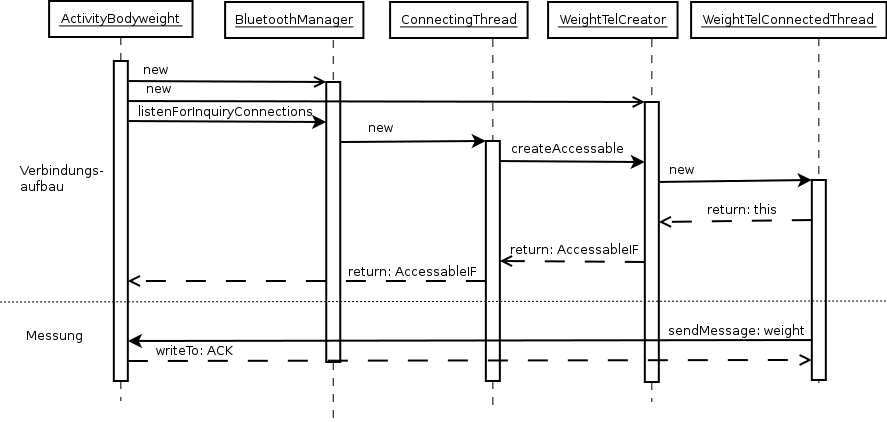
\includegraphics[scale=0.5]{diagramme/kapitel4/sequenzdiagramme/bt_com_aufbau_datasend.png}
  \caption{Sequenzdiagramm f\"ur Bluetoothverbindung und Datenaustausch}
  
\end{figure}

\subsection{Dekodieren einer Messung}

Das Dekodieren einer Messung wird am Beispiel der K\"orpergewichtsmessung erkl\"art.
Um eine Messung zu bekommen, muss zuerst das Protokoll der BodyTel-Ger\"ate erf\"ullt werden.
Der Ablauf dabei sieht folgenderma\ss{}en aus:
\begin{itemize}
 \item Sensor sendet: ATE0\\
 Das ist ein Echo und pr\"uft, ob jemand antwortet.
 \item ApoCo sendet: \textbackslash n \textbackslash r OK \textbackslash n \textbackslash r\\
 Antwort auf das Echo.
 \item Sensor sendet: AT+CMGS=142\\
 Das Kommando vor dem Gleichheitszeichen bedeutet, es wird eine Nachricht gesendet 
 und die Zahl danach ist die L\"ange der SMS.
 \item Sensor sendet: Nachricht als Hexadezimalzahlen.
 \item ApoCo sendet: \textbackslash r \textbackslash n +CMGS\\
 Best\"atigung der Nachricht.
\end{itemize}
Ende der Kommunikation.\\

Ab jetzt muss die Nachricht dekodiert werden. 
Daf\"ur veranschaulicht die Abbildung 4.6 in einem Klassendiagramm, welche Klassen f\"ur diesen Vorgang notwendig sind.

\begin{figure}[h]
  \centering
  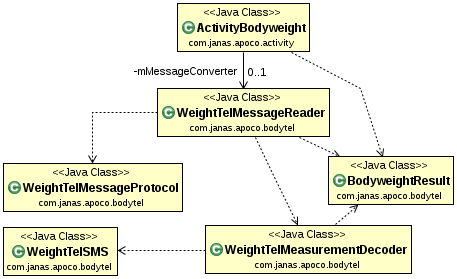
\includegraphics[scale=0.78]{diagramme/kapitel4/uml/weighttel_messagedecode.png}
  \caption{Klassendiagramm f\"ur Dekodieren von Nachrichten}
  
\end{figure}

Zum Einlesen der ankommenden Nachricht benutzt die Klasse \emph{ActivityBodyweight} ein Objekt der 
Klasse \emph{WeightTelMessageReader}.
Die Klasse \emph{WeightTelMessageReader} analysiert  die Nachricht und setzt die einzelnen ankommenden Bl\"ocke in einem St\"uck zusammen.
W\"ahrend der Analyse ordnet die Klasse \emph{WeightTelMessageReader} die richtigen Antwort-Strings zu, 
die an den Sensor zur\"uckgegeben werden.
F\"ur diese Analyse stehen in der Klasse \emph{WeightTelMessageProtocol} die entsprechenden Konstanten bereit.
Wurde die Nachricht zum Ende gelesen, wird die SMS als String an die Klasse \emph{WeightTelMeasurementDecoder} weitergereicht.
Hier wird die Methode \emph{decodeMeasurement()} aufgerufen.
Die Klasse \emph{WeightTelMeasurementDecoder} erzeugt ein Objekt vom Typ \emph{WeightTelSMS} und initialisiert es mit dem SMS-String.
Im Konstruktor der Klasse \emph{WeightTelSMS} wird der SMS-String an entsprechenden Stellen getrennt und in lesbare Werte umgewandelt.
Nach diesem Vorgang erzeugt die Klasse \emph{WeightTelMeasurementDecoder} ein Objekt von Typ \emph{BodyweightResult} und 
initialisiert es mit den Messergebnissen aus dem \emph{WeightTelSMS}-Objekt.
Das \emph{Result}-Objekt wird anschlie\ss{}end an die Activity durchgereicht.
Dieser Vorgang wird durch das Sequenzdiagramm in der Abbildung 4.7 verdeutlicht.\\

\begin{figure}[h]
  \centering
  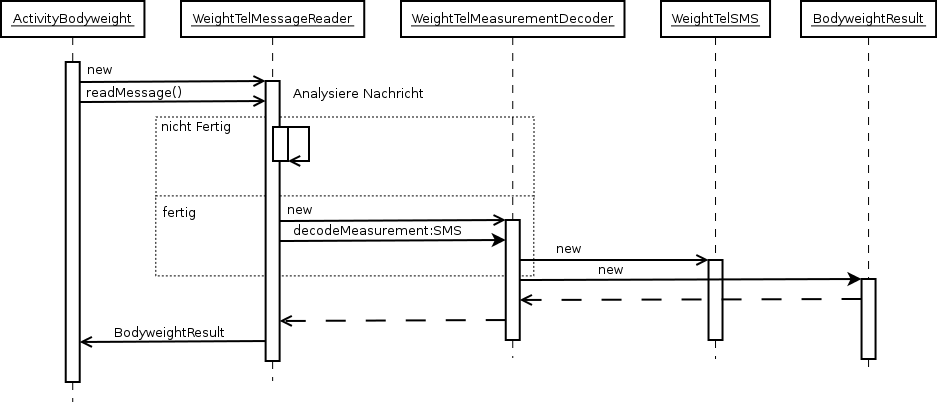
\includegraphics[scale=0.45]{diagramme/kapitel4/sequenzdiagramme/weighttel_messagedecode.png}
  \caption{Sequenzdiagramm f\"ur Dekodieren von Nachrichten}
  
\end{figure}

\subsection{Anzeigen und Speichern der Messwerte}

Nach einer Messung erscheint der neue Messwert ganz oben in einer ListView der Activity und wird anschlie\ss{}end 
in der Datenbank gespeichert.
Das funktioniert folgenderma\ss{}en:
Wenn das \emph{Result}-Objekt nach dem Dekodieren der SMS an die Activity durchgegeben wurde, 
erzeugt der Handler der Activity ein \emph{DTO}-Objekt.
Im Fall der K\"orpergewichtsmessung ist das ein Objekt der Klasse \emph{BodyweightDTO}.
Dieses Objekt wird mit dem \emph{Result}-Objekt initialisiert.
Nun wird aus dem \emph{DTO}-Objekt mit Hilfe der static Methode \emph{\texttt{convertDTO\_to\_MODEL()}} 
der Klasse \emph{BodyweightModel}, ein Objekt
der Klasse \emph{BodyweightModel}  erzeugt und an einen ArrayAdapter zum Anzeigen in der ListView \"ubergeben.
Das \emph{DTO}-Objekt wird durch die Klasse \emph{DBManagerLocal} in der Datenbank gespeichert.
Dieser Vorgang soll durch die Diagramme in den Abbildungen 4.8 und 4.9 nochmals verdeutlicht werden.


\begin{figure}[h]
  \centering
  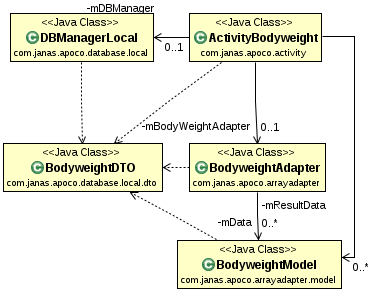
\includegraphics[scale=0.8]{diagramme/kapitel4/uml/show_results_in_lv.png}
  \caption{Klassendiagramm, Visualisierung und Speicherung der Daten}
  
\end{figure}

\begin{figure}[h]
  \centering
  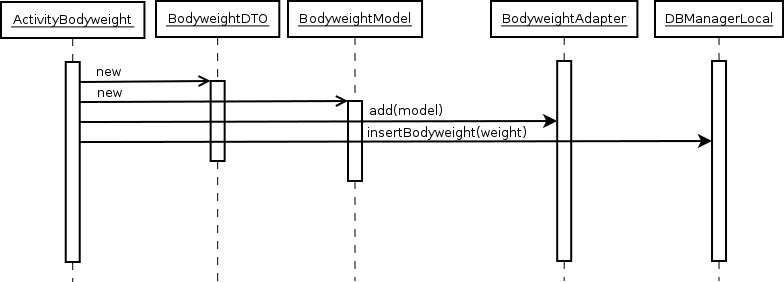
\includegraphics[scale=0.5]{diagramme/kapitel4/sequenzdiagramme/vl_db.png}
  \caption{Sequenzdiagramm, Visualisierung und Speicherung der Daten}
  
\end{figure}



\section{Datensynchronisation mit REST-Schnittstelle} 

\subsection{Datensynchronisation}

Nachdem die Messwerte aufgezeichnet sind, werden sie dem Arzt zug\"anglich gemacht.
So macht sich der Arzt ein Bild vom Zustand des Patienten und stellt eine Diagnose.
F\"ur diesen Zweck werden die Messprotokolle an einen Webserver gesendet.
Das Senden oder Synchronisieren startet immer wenn eine Activity beendet werden soll.
Als Beispiel wird die Activity f\"ur die Blutdruckmessung n\"aher betrachtet.
Damit das GUI nicht blockiert wird, muss das Synchronisieren immer nebenl\"aufig geschehen.
F\"ur diesen Zweck wird eine Klasse vom Typ AsyncTask genutzt.
Ein AsyncTask ist in drei Arbeitsbereiche aufgeteilt.
Im ersten Arbeitsbereich wird die Aufgabe noch im UI-Thread ausgef\"uhrt.
Daf\"ur ruft er seine Methode \emph{onPreExecute()} auf.
Hier kann der AsyncTask noch direkt auf die Activity zugreifen und die Aufgabe vorbereiten.
Im n\"achsten Schritt startet der AsyncTask einen eigenen Thread und f\"uhrt
die Aufgabe nun in seine \emph{doInBackground()}-Methode aus.
Das ist der nebenl\"aufige Teil der Ausf\"uhrung.
Ist dieser beendet, wird die Methode \emph{onPostExecute()} aufgerufen.
Er befindet sich wieder im UI-Thread.
Bevor ein AsyncTask beendet wird, werden hier noch die Ergebnisse an die Activity \"ubergeben.
Das Listing 4.9 zeigt eine reduzierte Form der \emph{SynchronizeBloodpressure}-Klasse, welche die Klasse
AsyncTask erweitert.
Die Messwerte werden mit einem AsyncTask gesendet.
Zuerst wird die Netzwerk- und Serververf\"ugbarkeit gepr\"uft.
Schl\"agt der Test fehl, so wird die Ausf\"uhrung beendet.
Als n\"achstes werden JSON-Objekte erzeugt, in denen die Messdaten abgelegt werden.
Im n\"achsten Schritt werden Tagesprotokolle, die noch nicht synchronisiert wurden, aus der Datenbank gelesen und
in JSON-Objekte gepackt.
Danach wird die URL zum Webserver zusammengebaut.
Dieser Vorgang ist wichtig, da zwar immer dieselbe IP genutzt wird, aber f\"ur jede Aufgabe wird ein anderes 
PHP-Skript vom Server aufgerufen.
Die PHP-Skripte bilden eine REST-Schnittstelle f\"ur die ApoCo-Anwendung.
Nachdem die URL bereitgestellt ist, wird eine Verbindung zum Webserver aufgebaut und ein 
\emph{HTTPRequest} ausgef\"uhrt.
Dabei werden die JSON-Strings mitgesendet.
Im letzten Schritt wird die Antwort vom Server ausgewertet und der 
Synchronisationsvorgang in der lokalen Datenbank best\"atigt.
Dabei wird das \emph{Sync}-Flag jeder synchronisierten Messung in der lokalen Datenbank auf den 
Wert 1 gesetzt und eine R\"uckmeldung an die Activity ausgegeben.
Der Synchronisationsvorgang wird in Abbildung 4.10 veranschaulicht.\\

\begin{figure}[h]
  \centering
  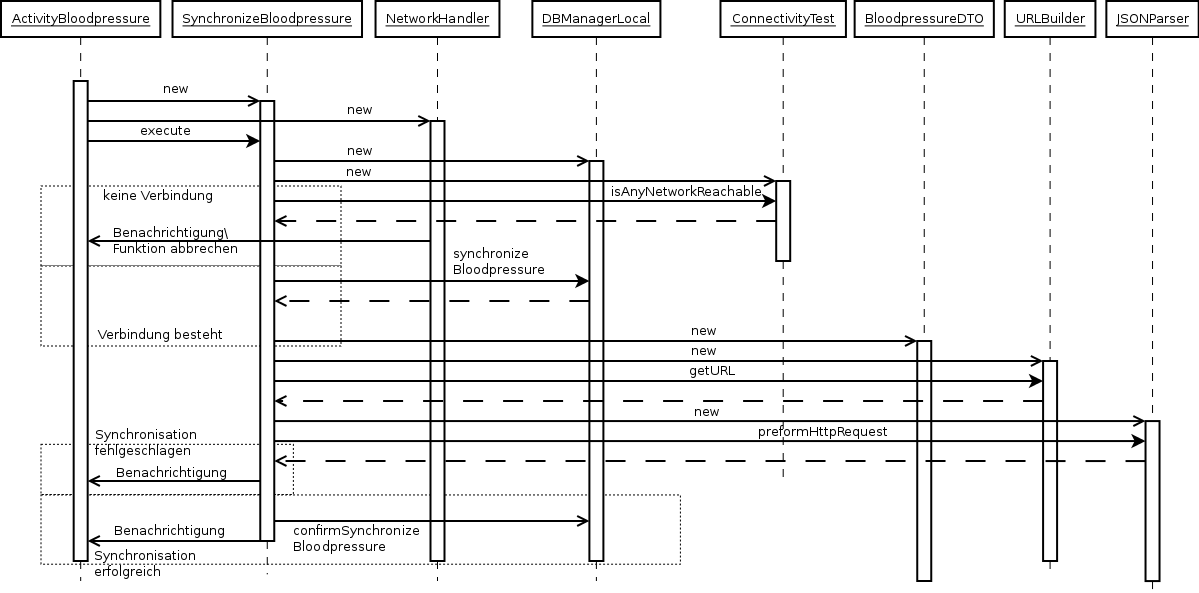
\includegraphics[scale=0.36]{diagramme/kapitel4/sequenzdiagramme/data_sync.png}
  \caption{Sequenzdiagramm f\"ur das Senden der Tagesprotokolle an den Webserver}
  
\end{figure}

\begin{lstlisting}[caption={SynchronizeBloodpressure sendet Blutdruckmesswerte an den Webserver}]
public class SynchronizeBloodpressure extends AsyncTask<UserDTO, Void, Boolean> {

   protected void onPreExecute() {
      ... /*Ablauf im UI-Thread*/
   } 
   /*ab hier startet ein neuer Thread*/
   protected Boolean doInBackground(UserDTO... pUser) {
      //Netzwerkverfuegbarkeit pruefen
      isNetworkConnected = new ConnectivityTest(mContext).isAnyNetworkReachable(mHandlerNet);
      if (!isNetworkConnected) return false;
      mUser = pUser[0];
      //JSON-Strukturen zum Senden werden angelegt
      JSONObject user = mUser.toJSONObject();
      JSONArray payload = new JSONArray();
      try {
         //Daten zum Synchronisieren aus der Datenbank laden
         Cursor cursor = mDBManager.synchronizeBloodpressure(mUser);
         while (cursor.moveToNext()) {
            //Daten in JSON-Strings verpacken
            BloodpressureDTO bpdto = new BloodpressureDTO(cursor);
            payload.put(cursor.getPosition(), bpdto.toJSONObject());
         }
      } catch (JSONException e) {}
      List<NameValuePair> params = new ArrayList<NameValuePair>();
      //JSON-String als Parameter fuer die Uebergabe an eine URL vorbereiten
      params.add(new BasicNameValuePair(JSON_TAG_IF.USER, user.toString()));
      params.add(new BasicNameValuePair(JSON_TAG_IF.PAYLOAD, payload.toString()));
      //aus Konfigurationsdaten die URL zusammenbauen
      String url = new URLBuilder().getURL(mContext, PHP_URL_IF.INSERT_BLOODPRESSURE);
      //HTTP-Anfrage an den Webserver senden
      jsonObject = new JSONParser().preformHttpRequest(url, JSONParser.RequestMethodE.POST, params);		
      try {
         //Antwort vom Webserver lesen
         int success = jsonObject.getInt(JSON_TAG_IF.SUCCESS);
         if (1 == success) {... return true;}
         else { return false;}
      }
    //Ende der Ausfuehrung, jetzt wieder im UI-Thread
    protected void onPostExecute(Boolean result) {
       if (result) {
       } else {
          //Nachricht kann direkt an die Activity uebergeben werden, hier geschieht es ueber ein Handler
          mHandlerAct.obtainMessage(ActivityBloodpressure.SYNCHRONIZING_DATA_COMPLETE).sendToTarget();
       }
       progressDialog.dismiss();
    }
}
\end{lstlisting}

\subsection{REST-Schnittstelle}

Die Rest-Schnittstelle auf dem Webserver ist aus mehreren PHP-Skripten aufgebaut.
Es gibt pro Funktionalit\"at ein Skript.
Die Persistenzschicht ist auf dem Webserver identisch modelliert, wie das in der Android-Anwendung der Fall ist.
Daf\"ur gibt es f\"ur jede Tabelle in der Datenbank eine entsprechende \emph{COLUMNS-, DTO-} und \emph{TBL-}Klasse.
Diese Klassen haben die gleiche Funktionalit\"at wie in der Android-Anwendung.
Sie beschreiben die Struktur und Tabellen der Datenbank als Objekte.
F\"ur die Verwaltung der Persistenzschicht ist die Klasse \emph{\texttt{DB\_Manager}} verantwortlich.
Dieser Manager baut bei Bedarf eine Verbindung zur Zieldatenbank auf und leitet die Anfragen an sie weiter.
Hier werden zwei unterschiedliche Datenbanken verwendet.
Eine geh\"ohrt zum Projekt \emph{ClearFood}.
Dort werden Informationen \"uber die Lebensmittel abgefragt.
Die andere Datenbank geh\"ohrt zu der Android-Anwendung ApoCo.
Hier werden die Messprotokolle aller Patienten gespeichert.
Wie eine Verbindung zur Datenbank gemacht wird, veranschaulicht das Listing 4.10.
Hier wird zum Aufbau der Kommunikation die Methode \emph{connect()} der Klasse \emph{\texttt{DB\_Manager}} gerufen.
Da die meisten Anfragen an die ApoCo-Datenbank gerichtet sind, 
wird hier standardm\"a\ss{}ig die Verbindung zu dieser Datenbank aufgebaut.\\

\begin{lstlisting}[caption={Verbindungsaufbau zur Datenbank}]
class DB_Manager {   
   private $db;   
   function connect() {
      $this->db = new mysqli(SERVER, USER, PASSWORD, DATABASE);
      return $this->db;
   }
}
//Verbindungsaufbau
$db = new DB_Manager();
$db->connect();
\end{lstlisting}

Die Anfragen sendet ApoCo an den Webserver \"uber HTTP.
Dabei wird f\"ur die gew\"unschte Anfrage ein PHP-Skript aufgerufen.
Eine solche Anfrage wird hier am Beispiel der Registrierung eines neuen Patienten im System veranschaulicht.
F\"ur das Registrieren wird das Skript \emph{register\texttt{\_}user.php} benutzt.
Der erste Schritt wird im Listing 4.11 demonstriert. 
Hier wird ein Array mit der Bezeichnung \emph{response} und ein Objekt der 
Klasse \emph{DB\texttt{\_}Manager} erstellt.
Das Array wird f\"ur die Antwort vom Server an die Android-Anwendung genutzt.\\

\begin{lstlisting}[caption={Benuzter registrieren, Schritt 1}]
$response = array();
$db = new DB_Manager();
\end{lstlisting}

Die Kommunikation zwischen ApoCo und Webserver wird hier durchgehend \"uber die HTTP-Methode POST gemacht.
Im n\"achsten Schritt werden mit der Funktion \emph{checkPOSTValues()} die Parameter in der 
Variablen POST auf G\"ultigkeit \"uberpr\"uft.
Die Methode \emph{checkPOSTValues()} wird im Listing 4.12 demonstriert.
Sind die empfangenen Parameter in Ordnung, wird die Abfrage ausgef\"uhrt.
Hat der Test fehlgeschlagen, wird eine entsprechende Nachricht als JSON-String zur\"uck an den Aufrufer gesendet.\\

\begin{lstlisting}[caption={Benuzter registrieren, Schritt 2}]
if (checkPOSTValues()) {
   //ok
} else {
   $response["success"] = 0;
   $response["message"] = "required field(s) is missing";
   echo json_encode($response);
}

function checkPOSTValues() {
   return isset($_POST[UserColumns::VORNAME]) &&
   isset($_POST[UserColumns::NACHNAME]) &&
   isset($_POST[UserColumns::EMAIL]) && 
   isset($_POST[UserColumns::PASSWORD]);
}
\end{lstlisting}

Sind die Parameter akzeptiert, so geht es mit dem n\"achsten Schritt weiter.
Mit der Klasse \emph{UserDto} wird aus den Parametern ein User-Objekt erzeugt.
Anschlie\ss{}end wird eine Verbindung zur Datenbank ge\"offnet.
Es wird gepr\"uft, ob die Email des neuen Benutzers bereits in der Datenbank vorhanden ist.
Ist das der Fall, wird seine Registrierung abgelehnt.
Handelt es sich dabei um keine bekannte Email, wird der neue Benutzer in die Datenbank aufgenommen 
und eine entsprechende positive R\"uckmeldung an den Aufrufer gesendet.
Diesen Vorgang veranschaulicht das Listing 4.13.\\

\begin{lstlisting}[caption={Benuzter registrieren, Schritt 3}]
$user = new UserDto($_POST);
$db->connect();
if($db->emailInUse($user->getEmail()) == 0) {
   $result = $db->registerNewUser($user);
   if($result) {
      $response["success"] = 1;
      $response["message"] = "user successfully registered";
      echo json_encode($response);
   } else {
      $response["success"] = 0;
      $response["message"] = "user registering failed";
      echo json_encode($response);
   }
} else { 
   $response["success"] = 0;
   $response["message"] = "email <" . $user->getEmail() . "> allready in use";
   echo json_encode($response);
}
\end{lstlisting}



\section{Barcodescanner} 

F\"ur die Berechnung der zugef\"uhrten Kilokalorien m\"ussen die Eigenschaften eines Lebensmittels erkannt werden.
Die Basis daf\"ur bildet der EAN-Code, der auf allen Nahrungsmitteln vorhanden ist.
Nachdem der EAN-Code gescannt wurde, ist der Software die EAN-Nummer bekannt.
Mit dieser Nummer wird in einer Datenbank nach einer \"Ubereinstimmung gesucht.
F\"ur die Projektumsetzung greift die ApoCo-Anwendung auf eine bereits existierende Datenbank aus dem Projekt 
\emph{ClearFood}.
ClearFood bietet alle notwendigen Informationen \"uber verschiedene Lebensmittel an.
Aus den Angaben \"uber Energiemenge pro 100g und dem gewogenen Gewicht wird die Energiemenge, 
die der Patient einnehmen m\"ochte, berechnet.\\
Zum Scannen des EAN-Codes wird die ZXing\cite{EAN:03}-Bibliothek genutzt.
ZXing wird \emph{zebra crossing} ausgesprochen. 
Es handelt sich dabei um eine Bibliothek f\"ur 1D und 2D Barcode-Bildverarbeitung.
Diese Bibliothek ist in Java implementiert und bietet eine Client-Anwendung f\"ur Android an.
Der ZXing-Client ist in ApoCo integriert.
Nach dem Start kann mit der Kamera auf der R\"uckseite des Smartphones ein Barcode erfasst werden.
Der ZXing-Client analysiert das Bild und gibt, nachdem ein Barcode erkannt wurde, 
diesen als EAN-Nummer an die ApoCo-Anwendung zur\"uck.
F\"ur diesen Zweck dienen die zwei Klassen \emph{IntentIntegrator} und \emph{IntentResult} im Paket \emph{zxing} 
der ApoCo-Anwendung.
Zudem muss das Manifest der Android-Anwendung modifiziert werden. 
Im Listing 4.14 wird die Integration der \emph{CaptureActivity}
aus der ZXing Bibliothek demonstriert.\\

\begin{lstlisting}[caption={ApoCo-Manifest, Integration von ZXing}]
//ApoCo_Manifest
...
 <activity 
            android:name="com.google.zxing.client.android.CaptureActivity"
            android:label="@string/app_name"
            android:screenOrientation="landscape">            
 </activity> 
\end{lstlisting}

\"Uber die Klasse \emph{ActivityMealenergy} wird der Barcodescanner verwendet.
Zum Starten dient hier die Klasse \emph{IntentIntegrator}.
Die Implementierung demonstriert das Listing 4.15.
Hier wird ein \emph{Integrator}-Objekt im \emph{OnClickListener} eines Buttons erzeugt.
Anschlie\ss{}end wird der Scan mit der Methode \emph{initiateScan()} gestartet.\\

\begin{lstlisting}[caption={Barcodesuche starten}]
barcodeScannerBTN.setOnClickListener(new OnClickListener() {
   IntentIntegrator ii = new IntentIntegrator(ActivityMealenergy.this);
   ii.initiateScan();
});
\end{lstlisting}

Der \emph{IntentIntegrator} bekommt im Konstruktor eine Referenz auf ein Objekt der 
Klasse \emph{ActivityMealenergy} \"ubergeben.
Nach der Initialisierung des Vorgangs bereitet er ein Intent zum eigentlichen Scan vor.
Anschlie\ss{}end wird das Intent als Parameter an die Methode \emph{startActivityForResult()} \"ubergeben,
welche \"uber die Referenz zur \emph{ActivityMealenergy} aufgerufen wird.
Ist der EAN-Code eingelesen, wird er an die Activity \emph{ActivityMealenergy} zur\"uckgegeben.
Das muss mit der Methode \emph{onActivityResult()} abgefangen werden.
Im Listing 4.16 wird das Abfangen demonstriert.\\

\begin{lstlisting}[caption={Ergebnis der Suche abfangen}]
protected void onActivityResult(int request, int result, Intent data) {
  super.onActivityResult(request, result, data);  
     switch(request) {
        case IntentIntegrator.REQUEST_CODE:
           if (RESULT_OK == result) {     
              //Ergebnis handhaben
              IntentResult r = IntentIntegrator.parseActivityResult(request, result, data);              
              String barcode = r.getContents();              
              Context activity = ActivityMealenergy.this;
              //GetFood ist ein AsyncTask zum Zugriff auf die Datenbank
              new GetFood(activity, new NetworkHandler(activity, true), mHandlerAct).execute(barcode);
           }
        break;
    }
}
\end{lstlisting}



\section{ApoCo Use Cases}

\subsection{Use Case- Diagramm}

Die Abbildung 4.11 veranschaulicht ein Use Case-Diagramm der ApoCo-Anwendung.
Hier werden Interaktionsm\"oglichkeiten des Benutzers mit der Android-Anwendung und die Kommunikation 
mit dem Webserver abgebildet.
\begin{figure}[h]
  \centering
  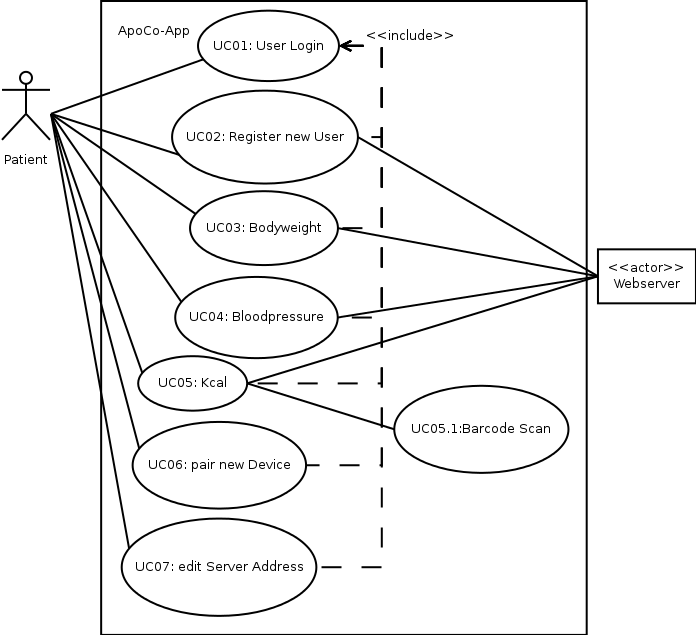
\includegraphics[scale=0.6]{diagramme/kapitel4/use_cases.png}
  \caption{ApoCo Use Case-Diagramm}
  
\end{figure}

\subsection{Aktoren}

\begin{itemize}
 \item Patient: Benutzer der ApoCo-Anwendung
 \item Webserver: Webserver mit Service zur Verwaltung der Tagesprotokolle
\end{itemize}

\subsection{Use Case Kurzbeschreibungen}

\begin{itemize}
 \item UC01: User Login\\ 
 Der Benutzer Meldet sich bei der ApoCo-Anwendung an.
 \item UC02: Register new User\\ 
 Ein neuer Benutzer registriert sich im System.
 Die Benutzerdaten werden zum Server gesendet und von diesem erlaubt oder verweigert.
 \item UC03: Bodyweight\\ 
 Der Benutzer f\"uhrt eine K\"orpergewichtsmessung durch.
 Zielgewicht wird vom Server geladen.
 Die Messung wird an den Server gesendet.
 \item UC04: Bloodpressure\\ 
 Der Benutzer f\"uhrt eine Blutdruckmessung durch.
 Die Messung wird an den Server gesendet.
 \item UC05: Kcal\\ 
 Der Benutzer f\"uhrt eine Protokollierung seiner Mahlzeit durch.
 Informationen zum Lebensmittel werden vom Webserver geladen.
 Mahlzeitprotokoll wird an den Server gesendet.
 \item UC05.1: Barcode Scan\\ 
 Der Benutzer scannt w\"ahrend einer Mahlzeitprotokollierung ein Lebensmittel mittels Barcodescanner ein.
 \item UC06: Pair new Device\\ 
 Der Benutzer f\"uhrt eine Ger\"ate-Koppelung durch.
 \item UC07: edit Server Address\\ 
 Der Benutzer konfiguriert die Webadresse des Servers.
\end{itemize} 




\section{ApoCo-GUI Gestaltung}

Die grafischen Elemente, wie Hintergrundbilder, farbige Buttons, Splashscreen, Farbgebung und das Logo,
sind mit einer Software f\"ur Bildbearbeitung und Illustration,
speziell f\"ur die Android-Anwendung designet.
Soweit es die Funktionalit\"at der einzelnen Activity zul\"asst, sind alle Activities identisch strukturiert.
Sie besitzen in diesem Fall immer die Elemente \emph{Header, Title, Body} und \emph{Footer}.
Das Einhalten der Struktur soll durch ein einheitliches Layout eine angenehme und einfache Bedienung der Software erm\"oglichen.
Die Abbildung 4.12 veranschaulicht und benennt die Hauptstrukturelemente einer Activity anhand der Start-Activity der ApoCo-Anwendung.\\

\begin{figure}[h]
  \centering
  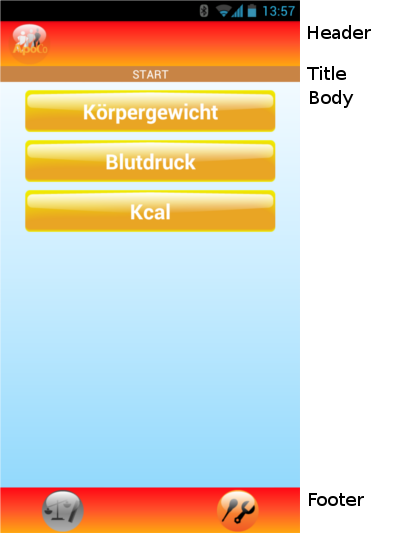
\includegraphics[scale=0.5]{screenshots/kapitel4/gui/activity_struktur.png}
  \caption{Start-Activity als Beispiel f\"ur Strukturierung}
  
\end{figure}

Die Strukturelemente haben jeweils eine eigene Funktion.
\begin{itemize}
 \item Header:\\
 Im \emph{Header} ist immer das ApoCo-Logo und wenn notwendig, ein \emph{Back-Button} angebracht.

 \item Title:\\
 Der \emph{Title} Bereich informiert den Benutzer auf welcher Activity er sich im Augenblick befindet.
 \item Body:\\
 Im \emph{Body} sind Interaktionselemente oder weitere notwendige Informationen der aktuellen Activity angebracht.
 Das k\"onnen Buttons zum Ansto\ss{}en von Messvorg\"angen oder ListViews sein.
 Eine ListView informiert den Benutzer \"uber alle bereits verzeichneten Messungen in der entsprechenden Activity.
 \item Footer:\\
 Am Ende der Activity ist der \emph{Footer}.
 Er beinhaltet Buttons, mit denen man in die Bereiche zum Ger\"ate-Koppeln, Sprung zur Start-Activity und zur 
 Server-Konfiguration gelangt. 
\end{itemize}


\subsection{Bedienelemente}

\subsubsection{Zur\"uck-Funktion}

Der Back-Button ist eines von mehreren M\"oglichkeiten, mit der ein Benutzer zu der vorherigen Activity zur\"uckkehren kann.
Einige davon haben lediglich die Funktion \emph{zur\"uck und Daten verwerfen} und andere wiederum 
\emph{zur\"uck und Daten speichern}.
Die Abbildung 4.13 veranschaulicht einen \emph{Header} mit \emph{Back-Button}.\\

\begin{figure}[h]
  \centering
  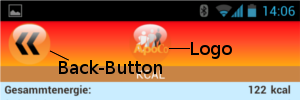
\includegraphics[scale=0.5]{screenshots/kapitel4/gui/header_backbtn.png}
  \caption{Header einer Activity mit \emph{Back-Button}}
  
\end{figure}

Die Abbildung 4.14 zeigt die Activity f\"ur Blutdruckmessung.
Mit Buchstaben sind hier alle M\"oglichkeiten der Software gekennzeichnet, die zur\"uck in die vorherige Activity f\"uhren.\\


\begin{figure}[h]
  \centering
  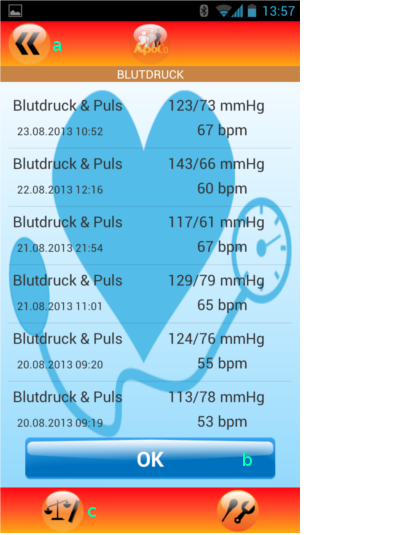
\includegraphics[scale=0.5]{screenshots/kapitel4/gui/back_btns.png}
  \caption{Zur\"uck-M\"oglichkeiten einer Activity}
  
\end{figure}


\begin{itemize}
 \item a) \emph{Back-Button}, Daten werden nicht gespeichert, zur\"uck zur vorherigen Activity. 
 \item b) \emph{OK-Button}, Daten werden gespeichert, anschlie\ss{}end zur\"uck zur vorherigen Activity.
 \item c) Sprung zur \emph{Start-Activity}, Daten werden nicht gespeichert. 
\end{itemize}

Neben einer Softwarem\"oglichkeit ist auch der Hardware-Button des Smartphones implementiert.
In der Abbildung 4.15 ist der Hardware-Button mit einem roten Kreis gekennzeichnet.
Hier findet kein Speichern der Daten statt.
Befindet man sich in der \emph{Start-Activity}, beendet ein Dr\"ucken auf die Hardware-Taste die ApoCo-Anwendung.\\

\begin{figure}[h]
  \centering
  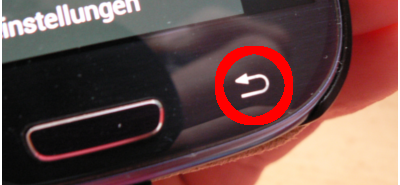
\includegraphics[scale=0.5]{screenshots/kapitel4/gui/hd_backbtn.png}
  \caption{Zur\"uck mit einem dem Hardware-Button des Smartphones}
  
\end{figure}

\subsubsection{Ger\"ateverwaltung}

In der Abbildung 4.16 ist der Button zur Ger\"ateverwaltung abgebildet.
Mit diesem Button gelangt man in den Bereich der Android-Anwendung, in welchen 
Messger\"ate gekoppelt und Servereinstellungen vorgenommen werden k\"onnen.

\begin{figure}[h]
  \centering
  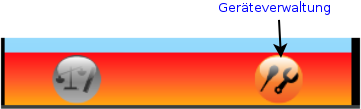
\includegraphics[scale=0.5]{screenshots/kapitel6/android/devices.png}
  \caption{Ger\"ateverwaltung}
  
\end{figure}

Die Abbildung 4.17 veranschaulicht anschlie\ss{}end die Activity der Ger\"ateverwaltung.
Hier wird \"uber Radio-Buttons eine Messung ausgew\"ahlt und \"uber eine der Koppelungsfunktionen
die externe Hardware verbunden.
Ob hier das Koppeln als Server oder Client gew\"ahlt wird, ist von dem externen Messsensor abh\"angig.\\

\begin{figure}[h]
  \centering
  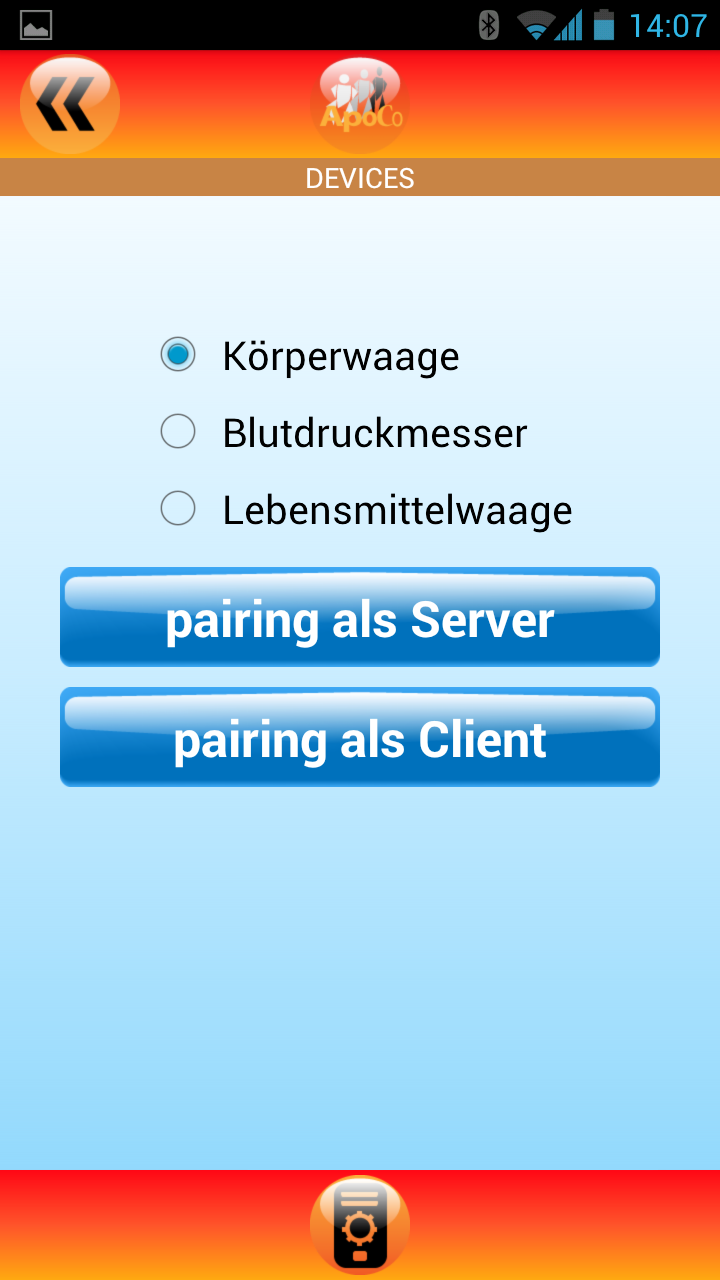
\includegraphics[scale=0.2]{screenshots/kapitel4/pairing.png}
  \caption{Koppelungsactivity}
  
\end{figure}

Im \emph{Footer}-Bereich der Abbildung 4.17 ist auch der Button f\"ur die Serverkonfiguration zu finden.
Die Serverkonfiguration wird mittels einer Activity realisiert, die sich allerdings im \emph{Dialog-Stil} pr\"asentiert.
Diese Aktivity wird in der Abbildung 4.18 veranschaulicht und das Listing 4.17 erl\"autert, 
wie man eine Activity \"uber das \emph{AndroidManifest} als Dialog erscheinen l\"asst.\\

\begin{figure}[h]
  \centering
  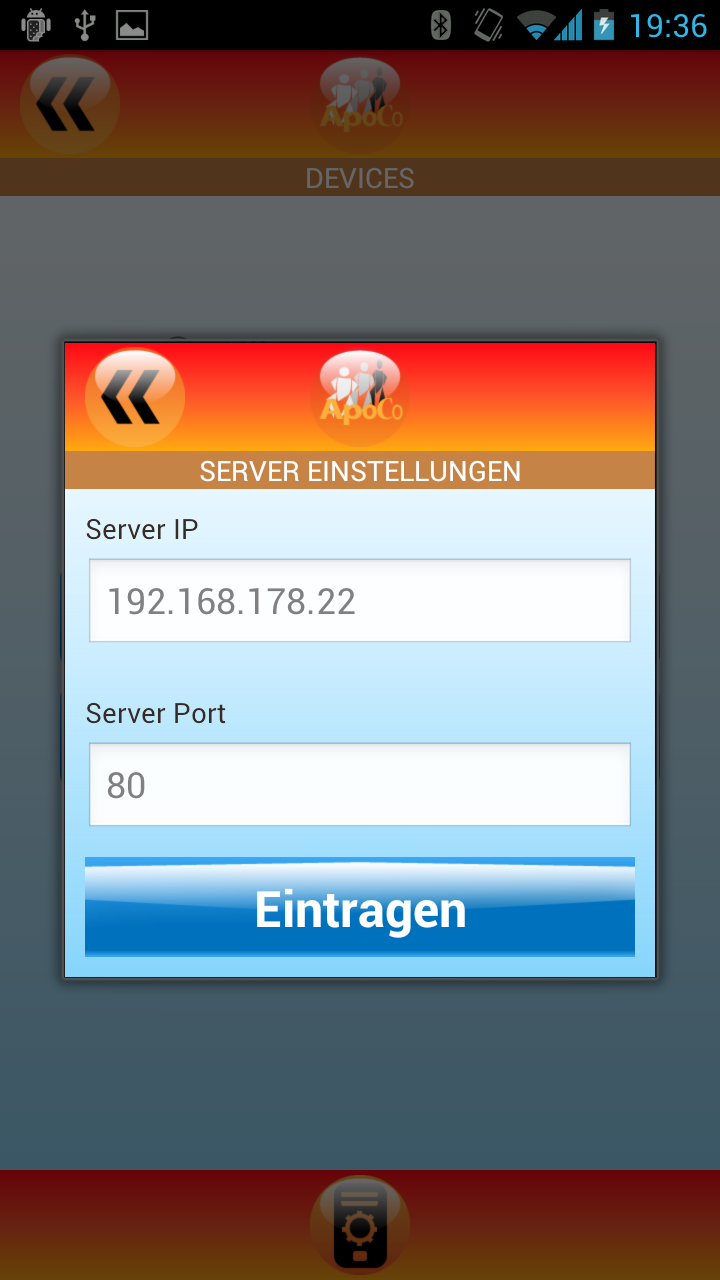
\includegraphics[scale=0.2]{screenshots/kapitel4/server_einstellungen.png}
  \caption{Serverkonfiguration}
  
\end{figure}

 \begin{lstlisting}[caption={Activity als Dialogfenster erscheinen lassen}]
 <activity
   android:name="com.janas.apoco.activity.ActivityServerOptions"
   //die zweite Zeile l\"asst die Activity als Dialog erscheinen
   android:theme="@android:style/Theme.Dialog" >
</activity>
\end{lstlisting}


\subsection{Activity-Wechsel mit Animation}

Der Wechsel von einer Aktivity zur anderen wird mit Animationsskripten gemacht.
Dabei wird die erste Activity zum Bildrand rausgezogen und die zweite Activity ins Bild hineingezogen.
Handelt es sich um den Wechsel zu einer Activity, die sich auf eine Parametrierung der Software bezieht, 
so verl\"auft die Animation von unten nach oben.
Wechselt man aber zur einer Messung, so verl\"auft die Animation von rechts nach links.
Eine vollst\"andige Animation besteht immer aus den zwei Teilen \emph{Eingangs-} und \emph{Ausgangs}-Animation.
Die Animationen sind im Odrner \emph{/res/anim/} in \emph{XML}-Dateien abgelegt.
Das Listing 4.18 veranschaulicht die Definition einer Animation und wie man sie f\"ur den Wechsel der Activities nutzt.\\

\begin{lstlisting}[caption={Animation zum Verlassen einer Activity}]
//rigt_side_in.xml
<?xml version="1.0" encoding="utf-8"?>
<set xmlns:android="http://schemas.android.com/apk/res/android" 
    android:interpolator="@android:anim/accelerate_decelerate_interpolator" >    
    <translate
        android:fromXDelta="100%p"
        android:toXDelta="0"
        android:duration="500"/>    
</set>
//Anwendung der Animation in einer Activity
finish();
overridePendingTransition(R.anim.left_side_in, R.anim.left_side_out);
\end{lstlisting}

Im Listing 4.18 ist ein Beispiel einer Animation f\"ur die reinkommende Activity zu sehen.
Durch den Aufruf der Methode \emph{overridePendingTransition()} wird eine Animation gestartet.
Diese Methode hat jedes Objekt vom Typ \emph{Activity}.
Sie muss zum Aufrufen \"uberschrieben werden.
Der Aufruf muss anschlie\ss{}end immer nach einer Methode erfolgen, welche f\"ur das Schlie\ss{}en einer Activity zust\"andig ist.
Das sind die Methoden \emph{finish()} und alle aus der Familie \emph{startActivity...()}.
Die Abbildung 4.19 zeigt zwei Screenshots mit jeweils einer Animation.
Bei der ersten ist der Wechsel in eine Messung zu sehen und in der zweiten zum Koppelungsvorgang.\\

\begin{figure}[h]
  \centering
  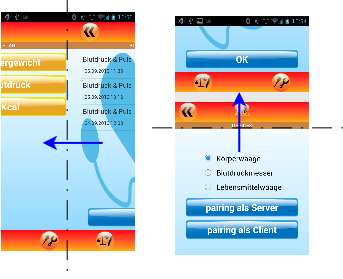
\includegraphics[scale=0.7]{screenshots/kapitel6/android/animation_richtung.png}
  \caption{\"Ubergangsanimation}
  
\end{figure}

\subsection{Views und Struktur der gegenseitigen Aufrufe}

In der Abbildung 4.20 ist die gesamte Viewschicht der Android-Anwendung veranschaulicht.
Die gro\ss{}en blauen Makierungen identifizieren die Views.
Wird ein Button gedr\"uckt, weist eine kleine blaue Makierung darauf hin, welche View als n\"achstes ge\"offnet wird.
Eine Ausnahme ist die View \emph{Splashscreen (s1)} und der Barcodescanner \emph{(b2)}.
Der \"Ubergang von Splashscreen zur Anmelde-View \emph{(a1)} geschieht \"uber einen Timer.
Ist der Timer abgelaufen, so startet der \"Ubergang automatisch.
Im Fall der Barcodescanner-View h\"angt der \"Ubergang davon ab,
ob nach dem Scan der Barcode in der Datenbank f\"ur Lebensmittel gefunden wurde oder nicht.
War die Suche erfolgreich, dann geht es mit der View \emph{(k3)} weiter.
Ist die Suche fehlgeschlagen, findet der \"Ubergang zur View \emph{(k2)} statt.\\

\begin{figure}[h]
  \centering
  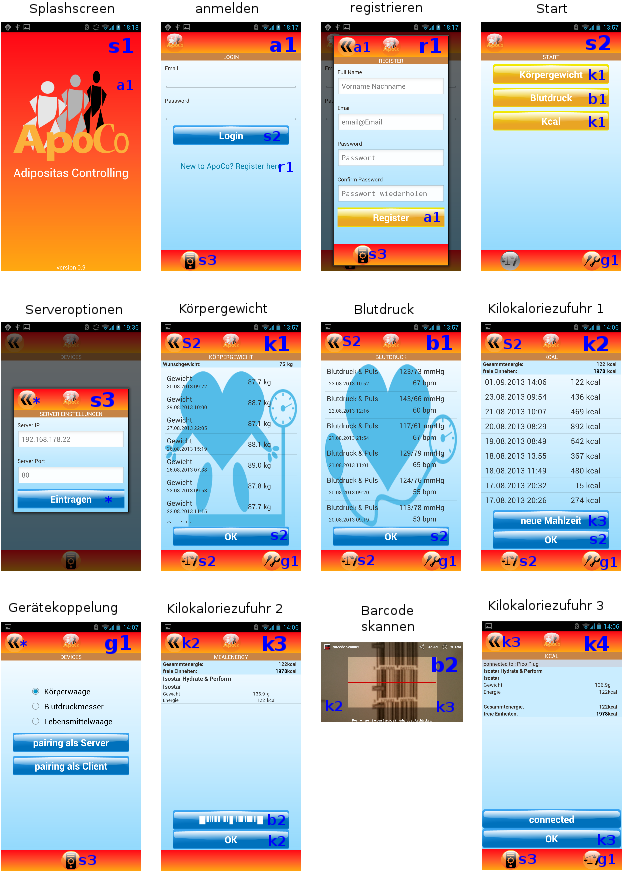
\includegraphics[scale=0.6]{diagramme/kapitel6/android/activity_map.png}
  \caption{Darstellung aller Activities}
  
\end{figure}

Um den Zusammenhang der Views besser darzustellen, 
zeigt die Abbildung 4.21 ein Zustandsdiagramm.
Dieses Zustandsdiagramm stellt die Beziehungen der Views untereinander dar.
Damit die Komplexit\"at des Diagramms \"uberschaubar bleibt,
wurde auf die Modellierung der Buttons f\"ur \emph{akzeptierende} und \emph{ablehnende} Aktionen verzichtet.
Im Diagramm sind nur die m\"oglichen \"Uberg\"ange zwischen den Views dargestellt.
Die Bezeichner der Zust\"ande im Diagramm entsprechen den Makierungen in der Abbildung 4.20, welche die Views identifizieren.
Zus\"atzlich sind die \"Ubergangspfade beschriftet und nummeriert.
Die Beschriftungen sagen aus, welche Aktion auf diesem Pfad vollzogen wird.
Die Nummerierungen bilden eine Hierarchie und sollen aufzeigen auf welche Weise ein Pfad verfolgt werden darf.
Es ist nur erlaubt einem wegf\"uhrenden Pfeil zu folgen, wenn der Pfad zuvor die gleiche Nummerierung hatte,
oder seine Nummerierung dem Folgepfeil als Pr\"afix vorangestellt ist.
Gelangt man \"uber einen Pfad zu einem verzweigenden Zustand,
dann wird die Nummerierung des letzten Pfeils
zum Pr\"afix der n\"achsten Pfade.\\
Betrachtet man den Zustand \emph{(r1)} in Abbildung 4.21.,
so ist es m\"oglich von \emph{(r1)} in den Zustand \emph{(s3)} hin und wieder zur\"uck zu wechseln.
Da keiner der restlichen Pfeile von \emph{(s3)} aus mit der 1 im Pr\"afix nummeriert ist, 
ist es beispielsweise nicht erlaubt von \emph{(s3)} nach \emph{(k4)} oder den \"ubrigen Zust\"anden zu wechseln.\\



\begin{figure}[h]
  \centering
  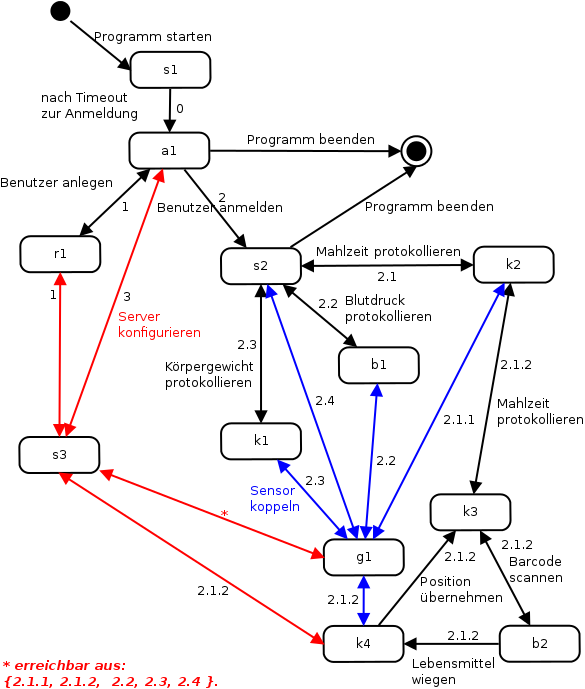
\includegraphics[scale=0.6]{diagramme/kapitel6/android/zustand_dialog_beziehung.png}
  \caption{Zustandsdiagramm f\"ur Beziehungen der gegenseitigen Aufrufe}
  
\end{figure}




